\documentclass[a4paper]{article}
\usepackage[letterpaper,margin=1in]{geometry}
\usepackage{blindtext}
\usepackage{lastpage}
\usepackage{fancyhdr}
\usepackage{setspace}
\usepackage{amsmath}
\usepackage{graphicx}
\usepackage{float}
\usepackage[small,bf,hypcap=true]{caption}
\newenvironment{Figure}
  {\par\medskip\noindent\minipage{\linewidth}%
   \captionsetup{type=figure}}
  {\endminipage\par\medskip}
\usepackage[hidelinks]{hyperref}
\usepackage{titlesec}
\usepackage{tocloft}

\renewcommand{\cftsecleader}{\cftdotfill{\cftdotsep}}

\graphicspath{{./Figures}}

% Configure the header
\pagestyle{fancy} % Enable fancy headers
\fancyhead[L]{CE 7029} % Left-aligned header
\fancyhead[C]{Numerical Modelling of Offshore Wind Turbines} % Centered header
\fancyhead[R]{-/03/2025} % Right-aligned header

\onehalfspacing

\begin{document}

\titleformat{\section}
  {\normalfont\bfseries\fontsize{12}{10}\selectfont}
  {\large\thesection.} 
  {0.3em}
  {}

\thispagestyle{empty}

\begin{figure}[H]
    \vspace{0.6cm}
    \centering
    
\includegraphics[width=0.45\textwidth]{logo.png}
\end{figure}
\vspace{0.8cm}

\begin{center}
    \textbf{\LARGE Middle East Technical University}
    \vspace{0.3cm}

    \textbf{\LARGE Department of Civil Engineering}
    \vspace{0.5cm}

    \textbf{\Large 2024-2025 Spring Semester}
    \vspace{1.5cm}

    \textbf{\Large CE 7029 Numerical Modelling of Offshore Wind Turbines}
    \vspace{0.9cm}

    \textbf{\Large Semester Project Report}
    \vspace{1.5cm}

    \large Instructor:

    \large Assoc. Prof. Dr. Elif Oğuz
    \vspace{1.2cm}

    \large Submitted by:
    
    \large Bilge Kutay

    \large 2511798

\end{center}

\newpage
\renewcommand{\contentsname}{Table of Contents} % Rename "Contents" to "Table of Contents"
\begin{center}
    \tableofcontents
\end{center}
\newpage

\section{Introduction}

\hspace*{0.5cm}The demand for renewable energy has driven significant advancements in offshore wind energy technologies, with floating offshore wind turbines (FOWTs) emerging as a practical solution for deep-water energy generation. This report focuses on the numerical modeling and analysis of the OC4 semisubmersible platform. 

The analysis of the OC4 semisubmersible platform was conducted using two approaches. Initially, simulations were performed using a pre-existing OC4 model in OpenFAST, a simulation tool for FOWTs, to analyze the platform's dynamic behavior under various load cases. These load cases, based on the methodology outlined in the study by Robertson et al. (2014), titled "Offshore Code Comparison Collaboration Continuation within IEA Wind Task 30: Phase II Results Regarding a Floating Semisubmersible Wind System," included free decay tests and wave-induced responses. The results were processed using BEMRosetta to extract natural frequencies and generate response graphs, which were compared to the reference study to validate the findings.

In addition to using the pre-existing OC4 model, the platform was also recreated independently using Rhino. The hydrodynamic properties of this recreated model were analyzed using HAMS to generate WAMIT output files, which were then converted into OpenFAST input files. The same load cases were applied to the recreated model in OpenFAST, allowing for a direct comparison between the pre-existing and recreated models. This approach provided a deeper understanding of the platform's performance and validated the modeling process.

This report provides a detailed account of the methodologies and results obtained during the numerical modeling and analysis of these floating offshore wind systems. By applying consistent load cases to both pre-existing and recreated models, the findings contribute to a comprehensive understanding of the dynamic behavior and performance of FOWTs under various conditions.

\section{OC4 Semisubmersible Platform Analysis}
\subsection{Article Review}
\hspace*{0.5cm}The study by Robertson et al. (2014) presents an analysis of the OC4 semisubmersible floating offshore wind system developed for the DeepCwind project (\autoref{fig:OC4}), comparing results from 21 different load cases (\autoref{tab:image_table}) simulated by 21 organizations using 19 distinct modeling tools. The research evaluates the platform’s dynamic behavior under progressively complex conditions, from basic system identification to combined environmental loads and damage scenarios. The study emphasizes the importance of accurate modeling in predicting the platform's response to environmental forces, including wind, waves, and currents. 

!!!RECONSIDER!!!!!!!
The most significant findings highlight that accurate platform modeling requires proper treatment of dynamic pressure effects on submerged members, particularly for heave motion. Nonlinear wave kinematics prove especially important for extreme wave conditions, where simplified approaches may fail to capture critical response characteristics. 
The study emphasizes the need for comprehensive validation of numerical models against experimental data, particularly in the context of floating wind turbine platforms. The results show the importance of considering various modeling approaches and their implications for predicting platform behavior under different environmental conditions.

This report focuses on the cases of free decay tests and wave-induced responses, which are crucial for understanding the platform's dynamic behavior. The free decay tests involve subjecting the platform to initial displacements and allowing it to oscillate freely, while the wave-induced responses are analyzed by applying regular and irregular waves to the platform and measuring its response in terms of heave, pitch, and surge motions.
The results of these tests provide valuable insights into the platform's natural frequencies and response characteristics, which are essential for designing and optimizing floating offshore wind systems.
\vspace{0.5cm}

\begin{figure}[htbp]
    \begin{minipage}{0.47\textwidth}
        \centering
        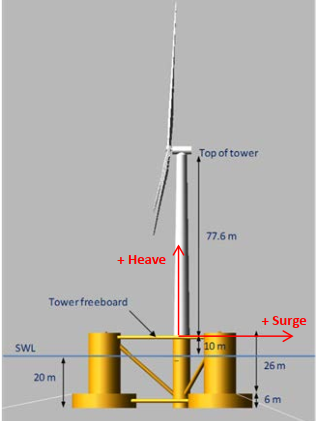
\includegraphics[width=0.93\textwidth]{OC4.png}
        \caption{\small OC4-DeepCwind floating wind system design. (Robertson et al., 2014)}
        \label{fig:OC4}
    \end{minipage}
    \hfill
    \begin{minipage}{0.5\textwidth}
        \centering
        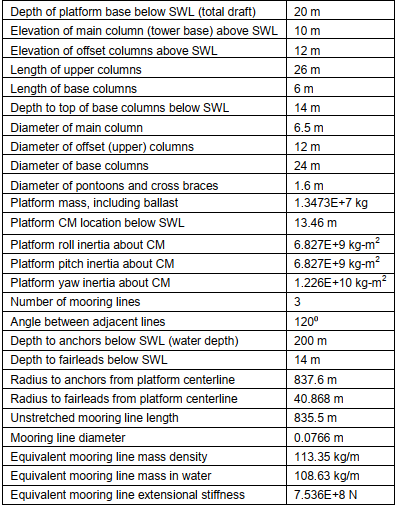
\includegraphics[width=0.9\textwidth]{characteristics.png}
        \caption{\small Summary of semisubmersible properties (Robertson et al., 2014)}
        \label{fig:characteristics}
    \end{minipage}
\end{figure}

\begin{table}[H]
    \centering
    \caption{Load cases run in OC4 Phase II. (Robertson et al., 2014)}
    \label{tab:image_table}
    \begin{tabular}{c}
        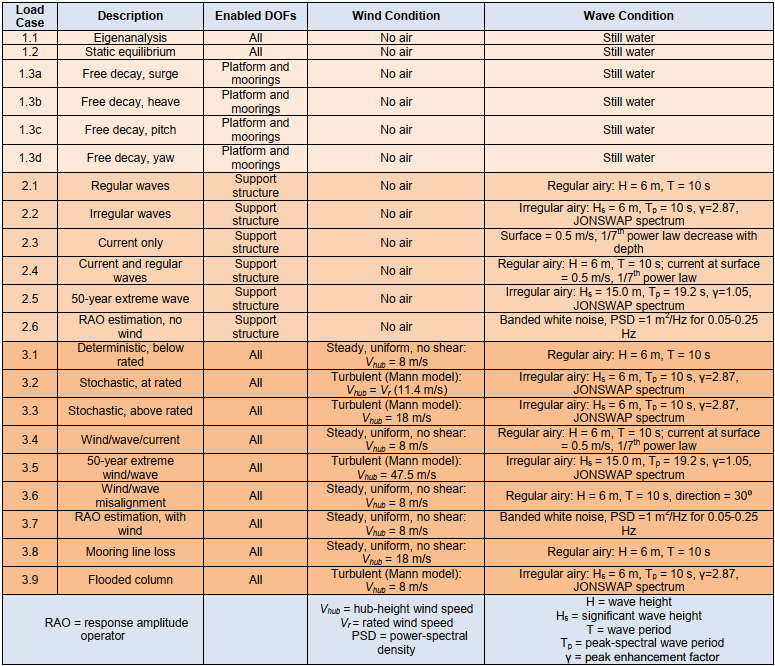
\includegraphics[width=0.95\textwidth]{table_3.png} \\
    \end{tabular}
\end{table}


\subsection{Pre-existing Model Analysis}

\hspace*{0.5cm}In this section, the analysis of the OC4 semisubmersible platform was conducted using a pre-existing model in OpenFAST called "5MW\_OC4Semi\_WSt\_WavesWN". The model was subjected to free decay and wave-induced load cases, namely Group 1.3X, 2.1, and 2.2, as outlined in the study by Robertson et al. (2014). The results were processed using BEMRosetta to extract natural frequencies and generate response graphs.

\subsubsection{Free Decay Tests}
\hspace*{0.5cm}The free decay tests involves subjecting the platform to initial displacements and allowing it to oscillate freely. Each of the four cases from 1.3a to 1.3d analyze the four individual degrees of freedom, specifically surge, heave, pitch, and yaw. The platform is given an initial displacement in the respective degree of freedom for each load case. The motion response of the platform was calculated using OpenFAST, and the natural frequencies were extracted from the time-domain data using the Fast Fourier Transform (FFT) method on BEMRosetta. The motion results of the 1.3a and 1.3b can be seen in Figures 4-14. The natural frequencies obtained from the tests for 6 degrees of freedom are shown in Figures 16-21 and consistent with the reference study, confirming the accuracy of the modeling approach \autoref{fig:nat_freq}.
\vspace{0.3cm}

%%1.3a figures
\begin{figure}[H]
    \begin{minipage}{0.48\textwidth}
        \centering
        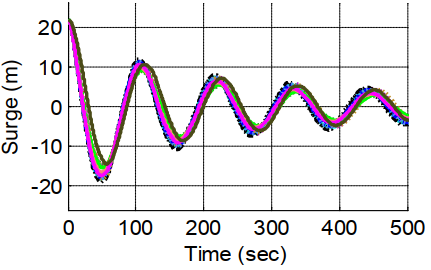
\includegraphics[width=0.97\textwidth]{1.3a_surge.png}
        \caption{\small Surge free decay platform motion response for 1.3a (Robertson et al., 2014)}
        \label{fig:1.3a_surge}
    \end{minipage}
    \hfill
    \begin{minipage}{0.49\textwidth}
        \centering
        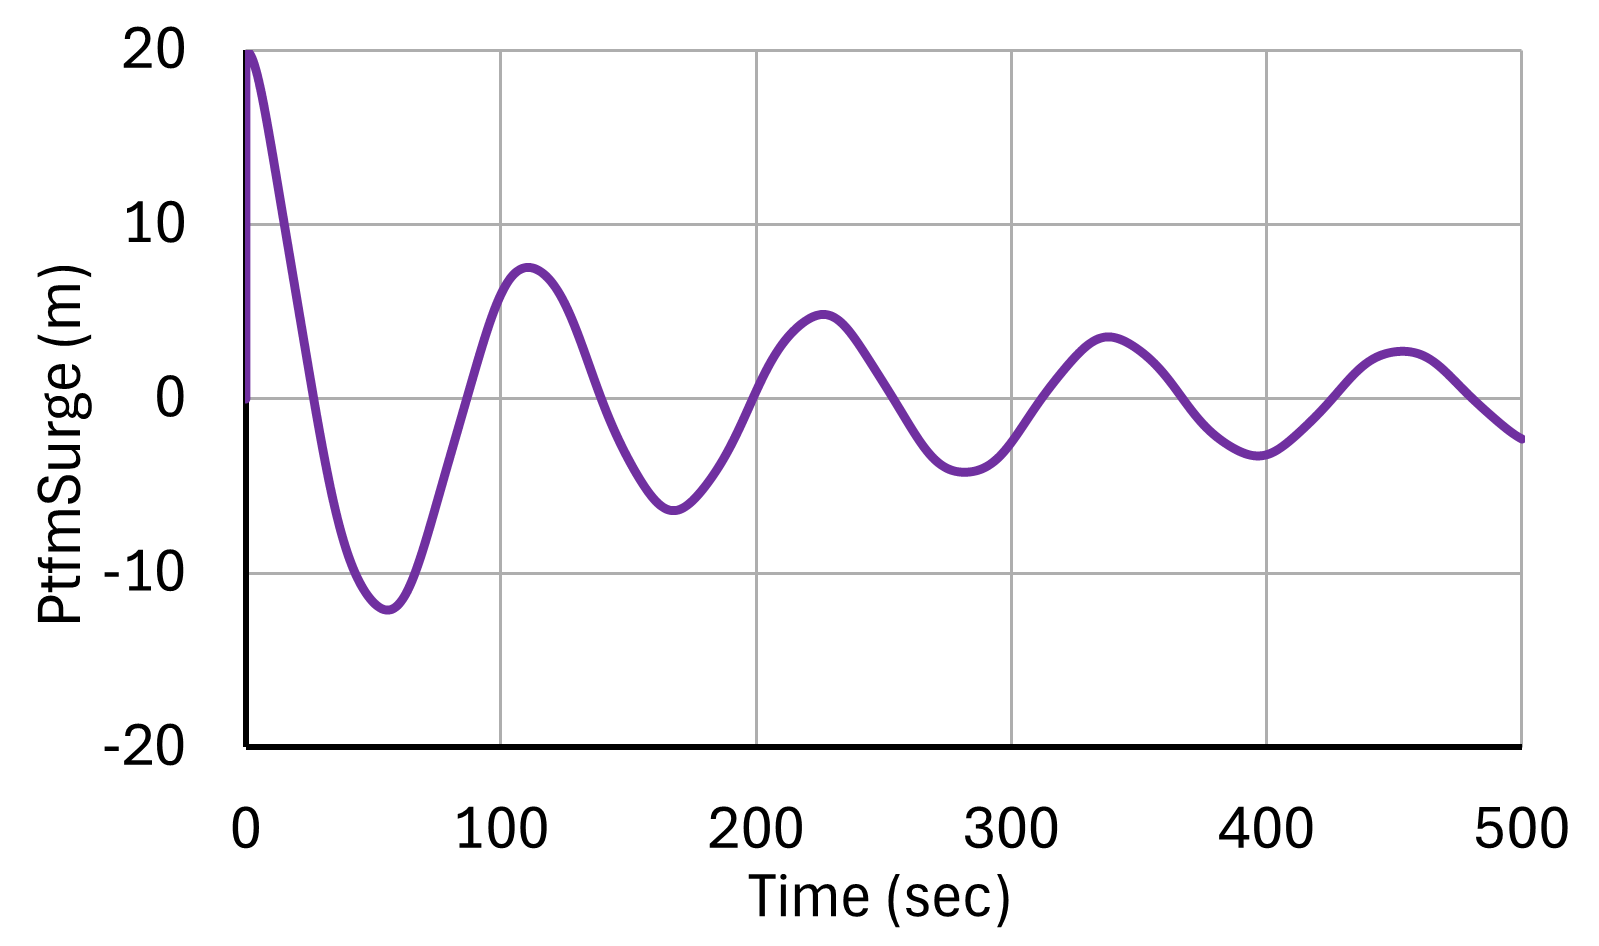
\includegraphics[width=1\textwidth]{1.3a_surge_mine.png}
        \caption{\small Surge free decay platform motion response for 1.3a}
        \label{fig:1.3a_surge_mine}
    \end{minipage}
\end{figure}

\begin{figure}[H]
    \begin{minipage}{0.48\textwidth}
        \centering
        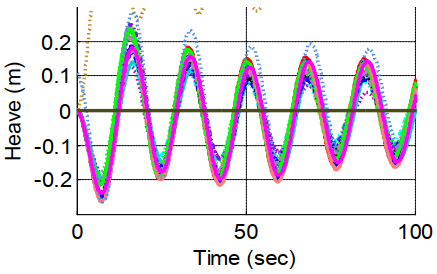
\includegraphics[width=0.97\textwidth]{1.3a_heave.png}
        \caption{\small Heave free decay platform motion response for 1.3a (Robertson et al., 2014)}
        \label{fig:1.3a_heave}
    \end{minipage}
    \hfill
    \begin{minipage}{0.49\textwidth}
        \centering
        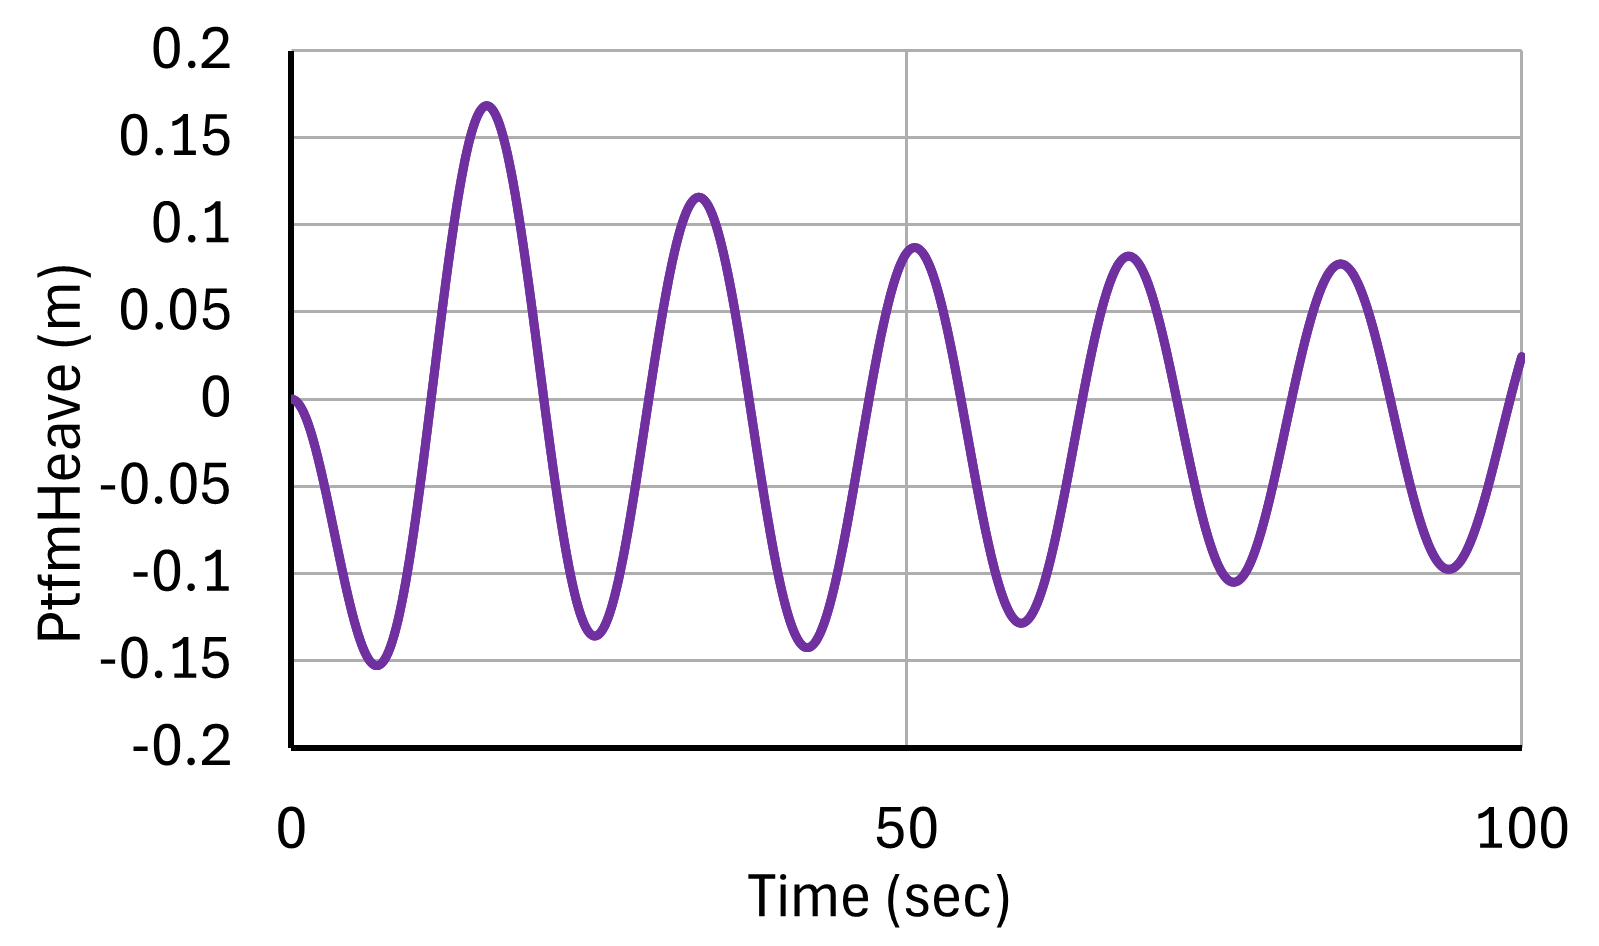
\includegraphics[width=1\textwidth]{1.3a_heave_mine.png}
        \caption{\small Heave free decay platform motion response for 1.3a}
        \label{fig:1.3a_heave_mine}
    \end{minipage}
\end{figure}

\begin{figure}[H]
    \begin{minipage}{0.48\textwidth}
        \centering
        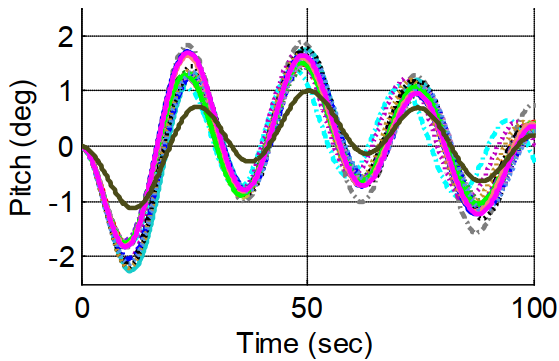
\includegraphics[width=0.97\textwidth]{1.3a_pitch.png}
        \caption{\small Pitch free decay platform motion response for 1.3a (Robertson et al., 2014)}
        \label{fig:1.3a_pitch}
    \end{minipage}
    \hfill
    \begin{minipage}{0.49\textwidth}
        \centering
        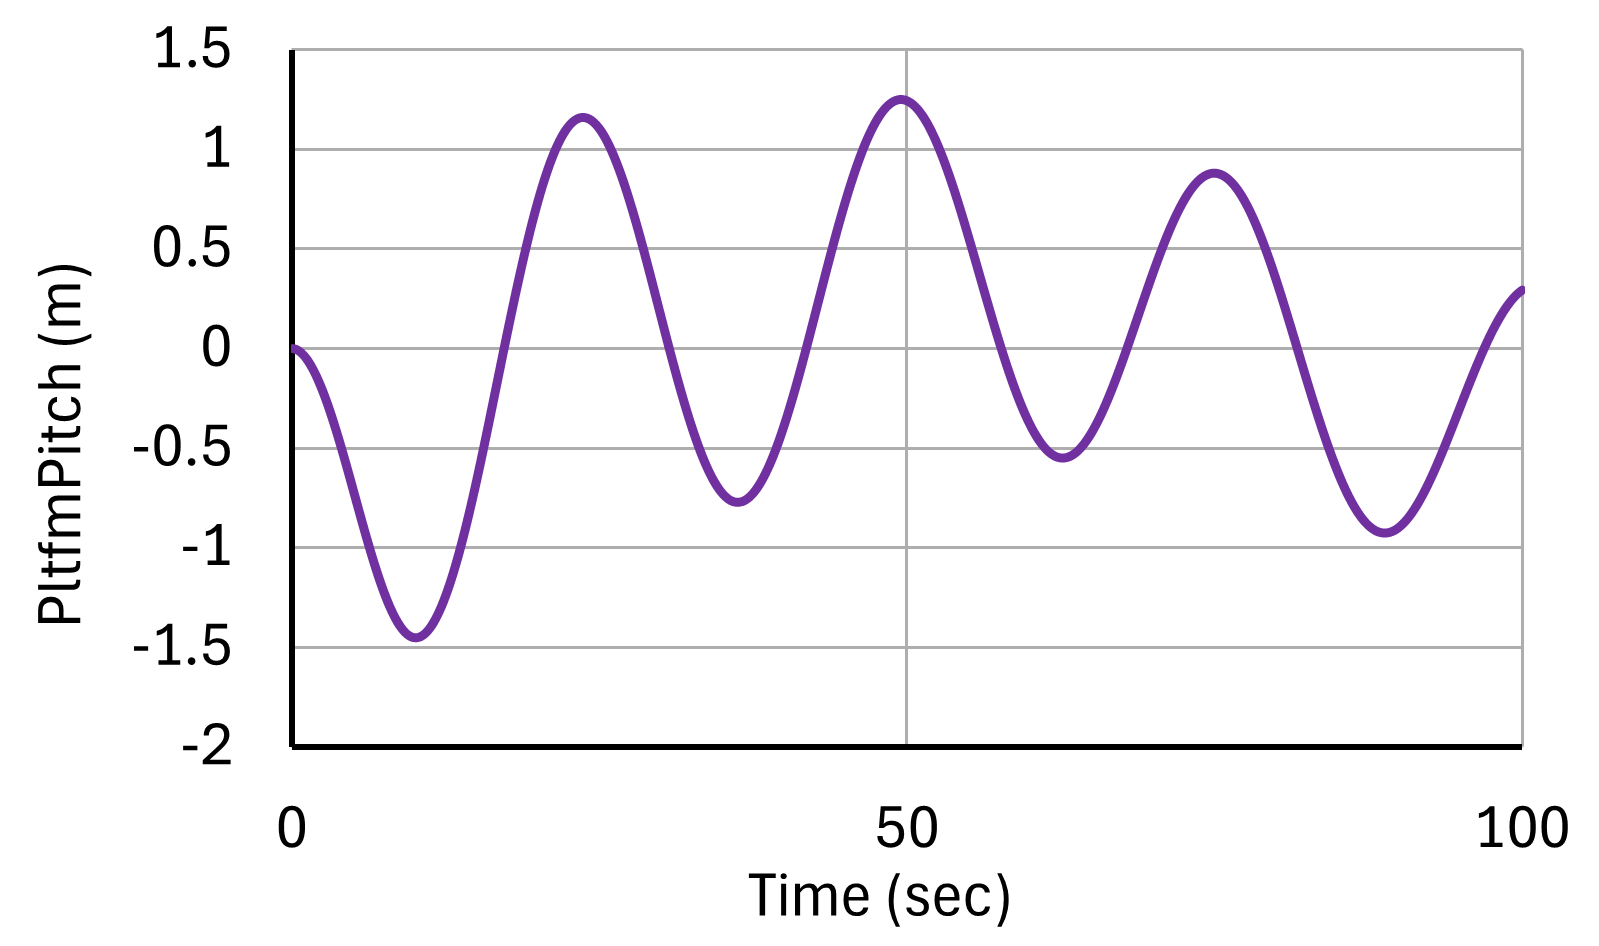
\includegraphics[width=1\textwidth]{1.3a_pitch_mine.png}
        \caption{\small Pitch free decay platform motion response for 1.3a}
        \label{fig:1.3a_pitch_mine}
    \end{minipage}
\end{figure}

%%1.3b figures
\begin{figure}[H]
    \begin{minipage}{0.47\textwidth}
        \centering
        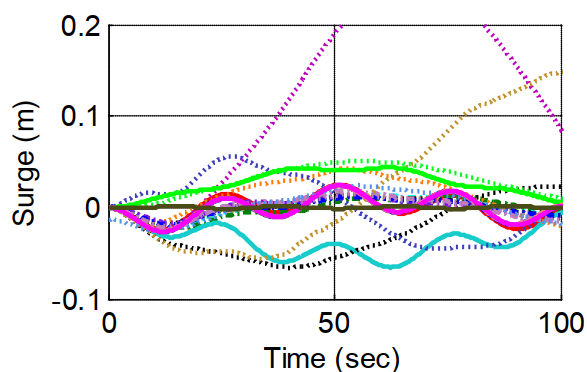
\includegraphics[width=0.97\textwidth]{1.3b_surge.png}
        \caption{\small Surge free decay platform motion response for 1.3b (Robertson et al., 2014)}
        \label{fig:1.3b_surge}
    \end{minipage}
    \hfill
    \begin{minipage}{0.5\textwidth}
        \centering
        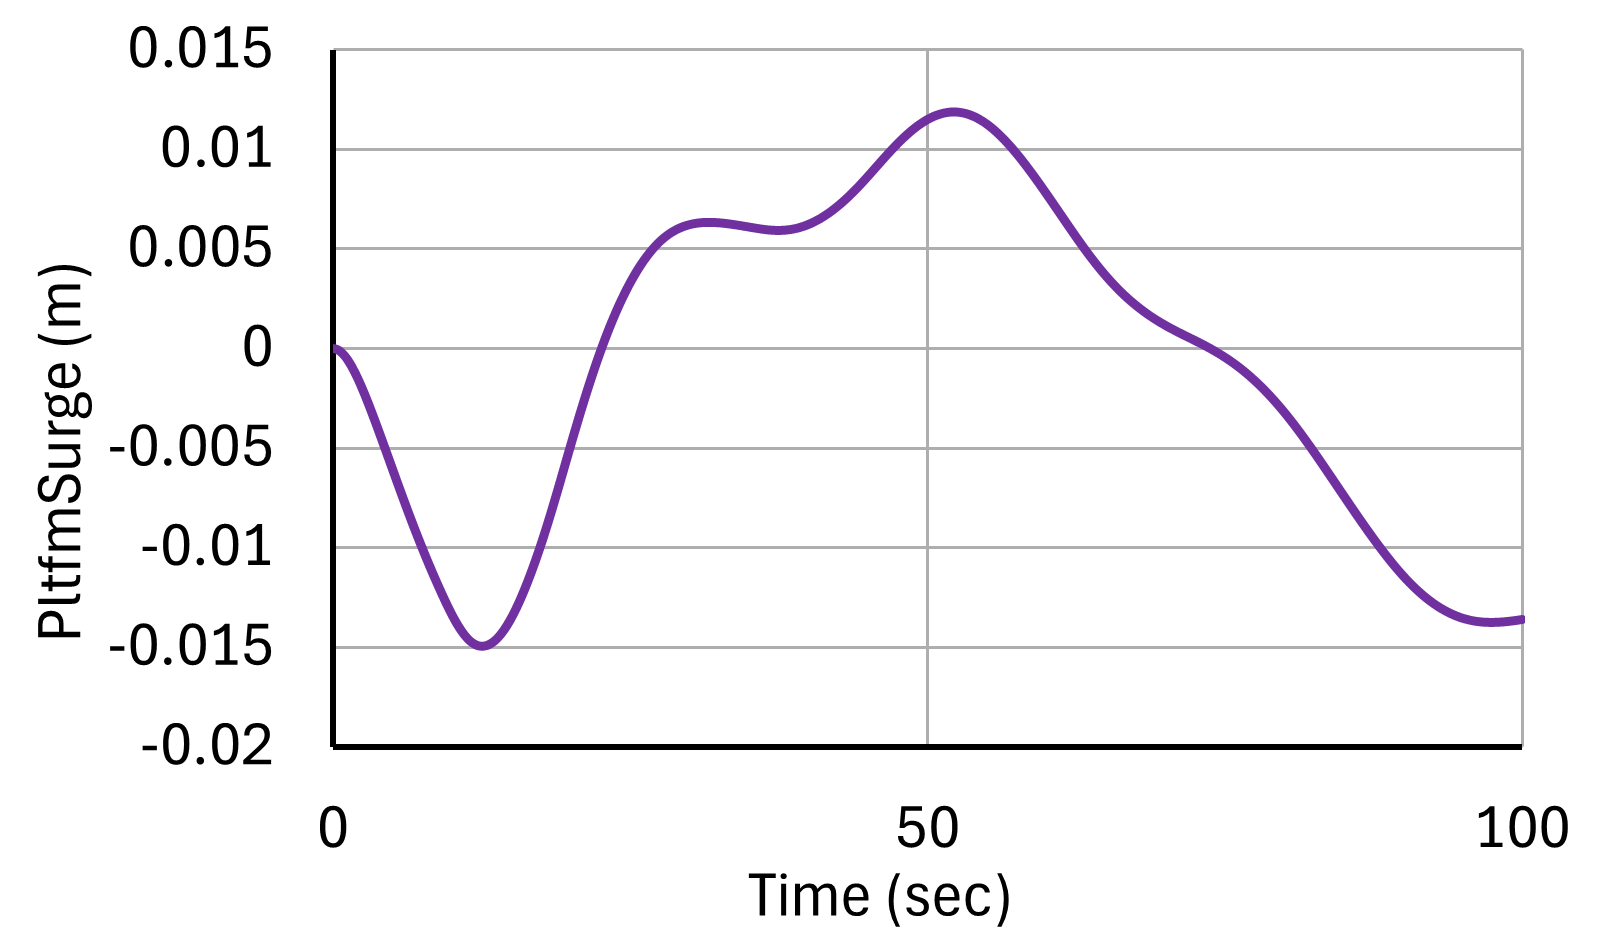
\includegraphics[width=1\textwidth]{1.3b_surge_mine.png}
        \caption{\small Surge free decay platform motion response for 1.3b}
        \label{fig:1.3b_surge_mine}
    \end{minipage}
\end{figure}

\begin{figure}[H]
    \begin{minipage}{0.47\textwidth}
        \centering
        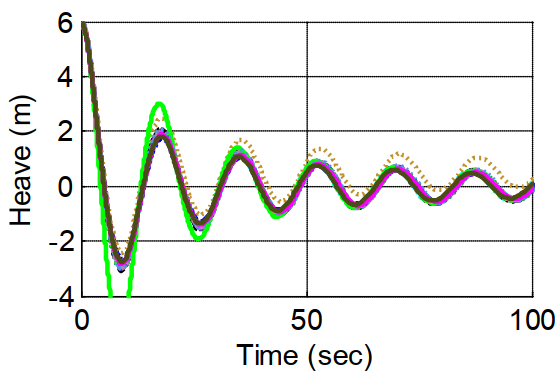
\includegraphics[width=0.97\textwidth]{1.3b_heave.png}
        \caption{\small Heave free decay platform motion response for 1.3b (Robertson et al., 2014)}
        \label{fig:1.3b_heave}
    \end{minipage}
    \hfill
    \begin{minipage}{0.5\textwidth}
        \centering
        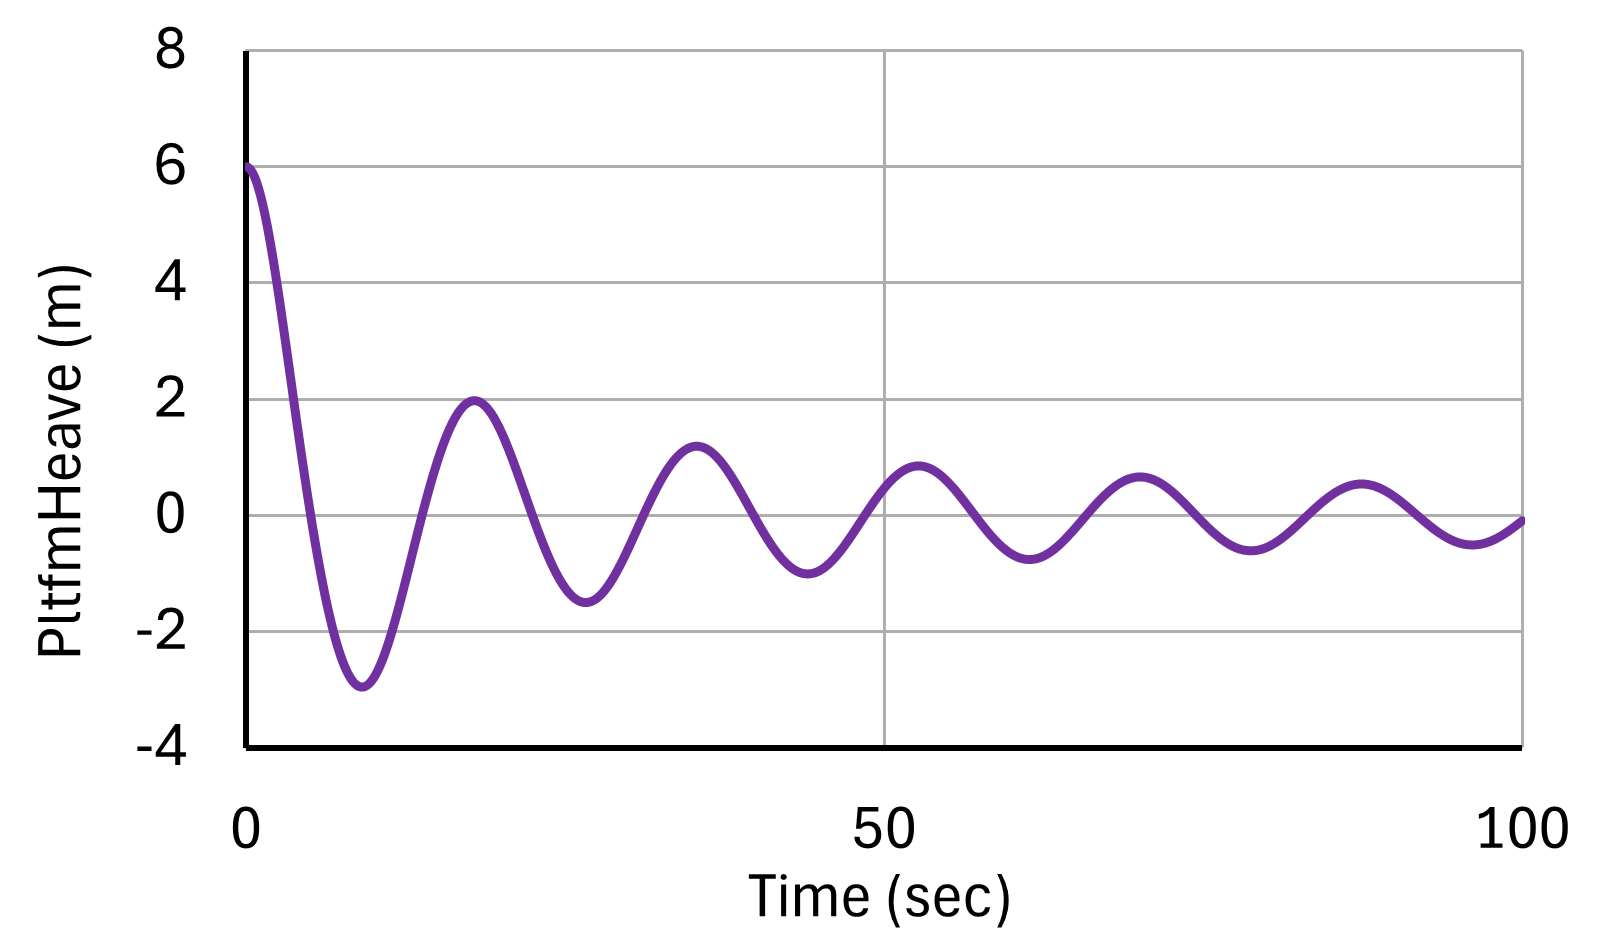
\includegraphics[width=1\textwidth]{1.3b_heave_mine.png}
        \caption{\small Heave free decay platform motion response for 1.3b}
        \label{fig:1.3b_heave_mine}
    \end{minipage}
\end{figure}

\begin{figure}[H]
    \begin{minipage}{0.47\textwidth}
        \centering
        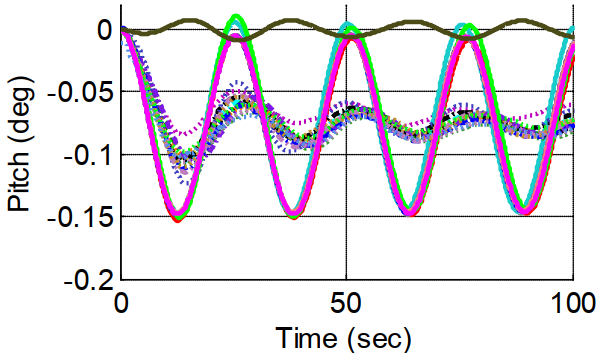
\includegraphics[width=0.97\textwidth]{1.3b_pitch.png}
        \caption{\small Pitch free decay platform motion response for 1.3b (Robertson et al., 2014)}
        \label{fig:1.3b_pitch}
    \end{minipage}
    \hfill
    \begin{minipage}{0.5\textwidth}
        \centering
        \vspace{-0.3cm}
        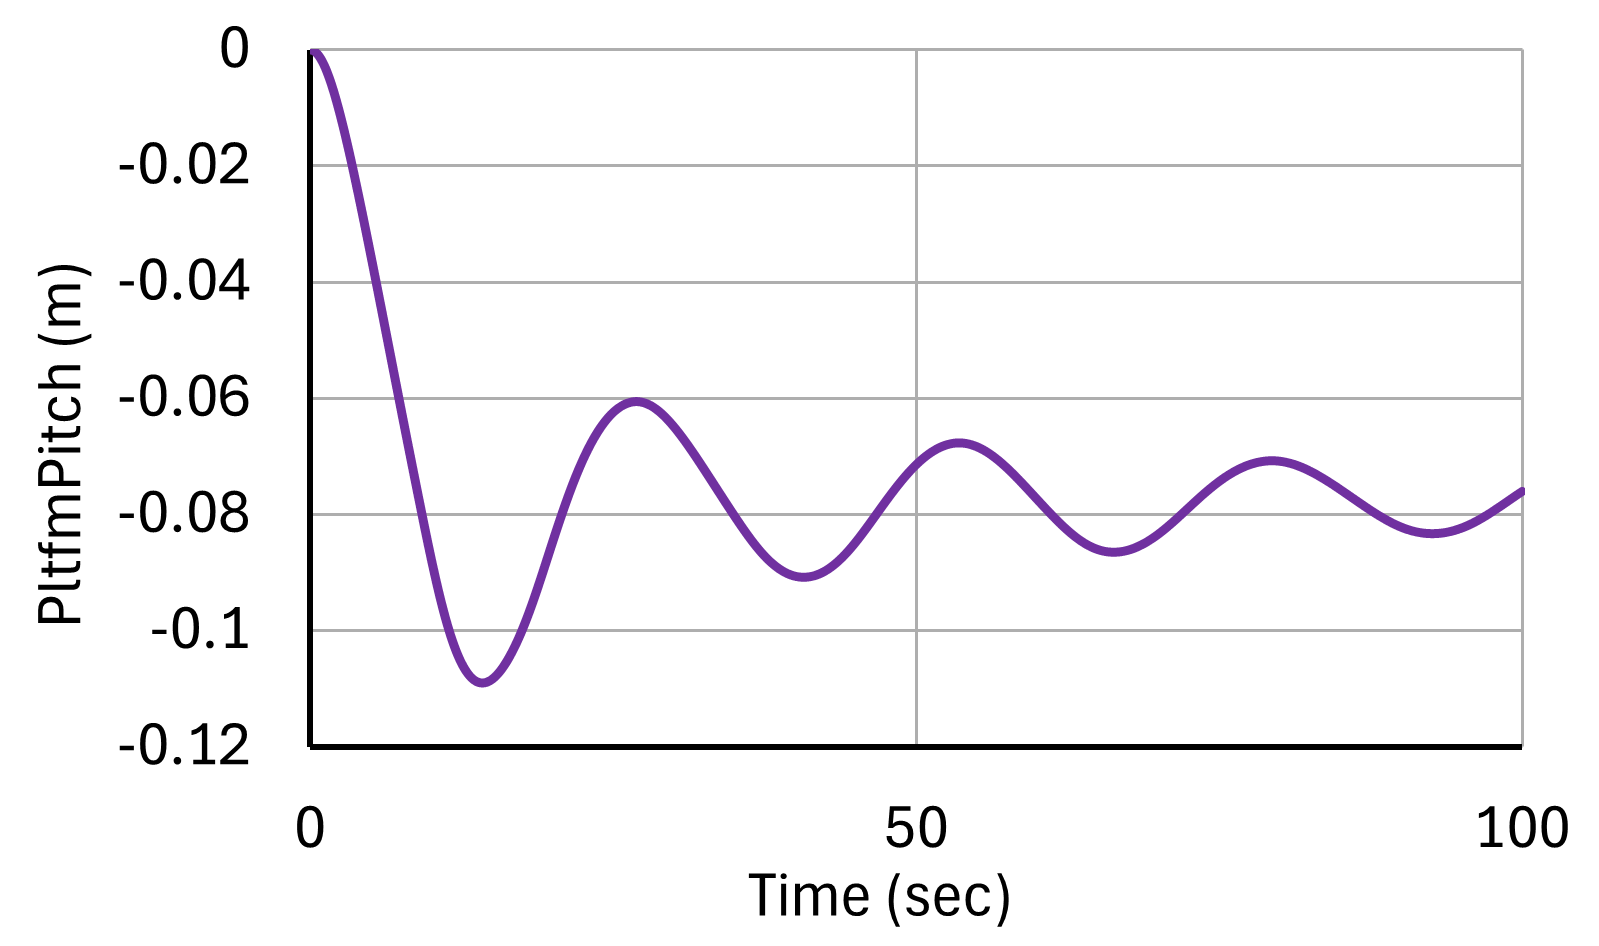
\includegraphics[width=1\textwidth]{1.3b_pitch_mine.png}
        \caption{\small Pitch free decay platform motion response for 1.3b}
        \label{fig:1.3b_pitch_mine}
    \end{minipage}
\end{figure}

%%natural frequencies

\begin{figure}[H]
    \centering
    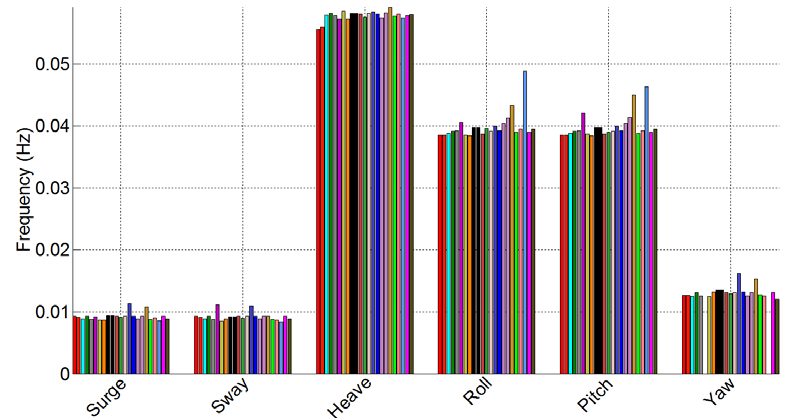
\includegraphics[width=0.9\textwidth]{nat_freq.png}
    \caption{\small Full-system natural frequencies (Robertson et al., 2014)}
    \label{fig:nat_freq}
\end{figure}

\begin{figure}[H]
    \begin{minipage}{0.49\textwidth}
        \centering
        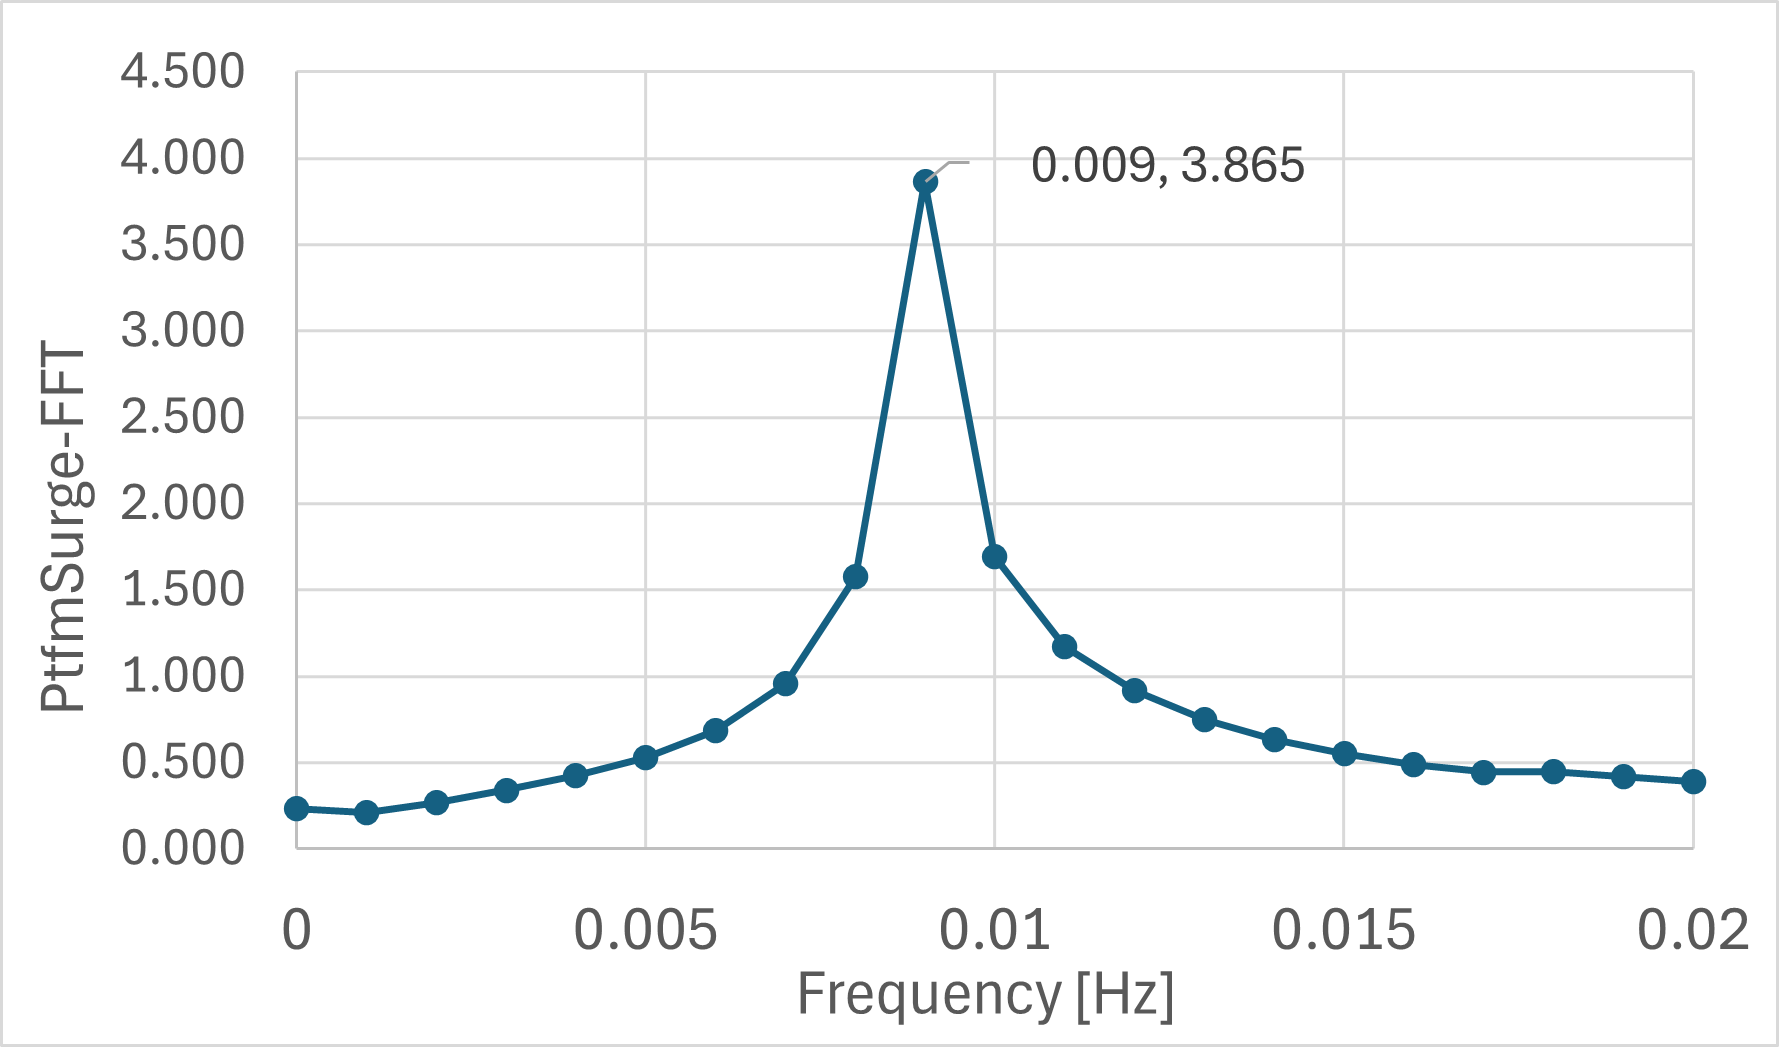
\includegraphics[width=1\textwidth]{nat_freq_surge.png}
        \caption{\small Surge natural frequency}
        \label{fig:nat_freq_surge}
    \end{minipage}
    \hfill
    \begin{minipage}{0.5\textwidth}
        \centering
        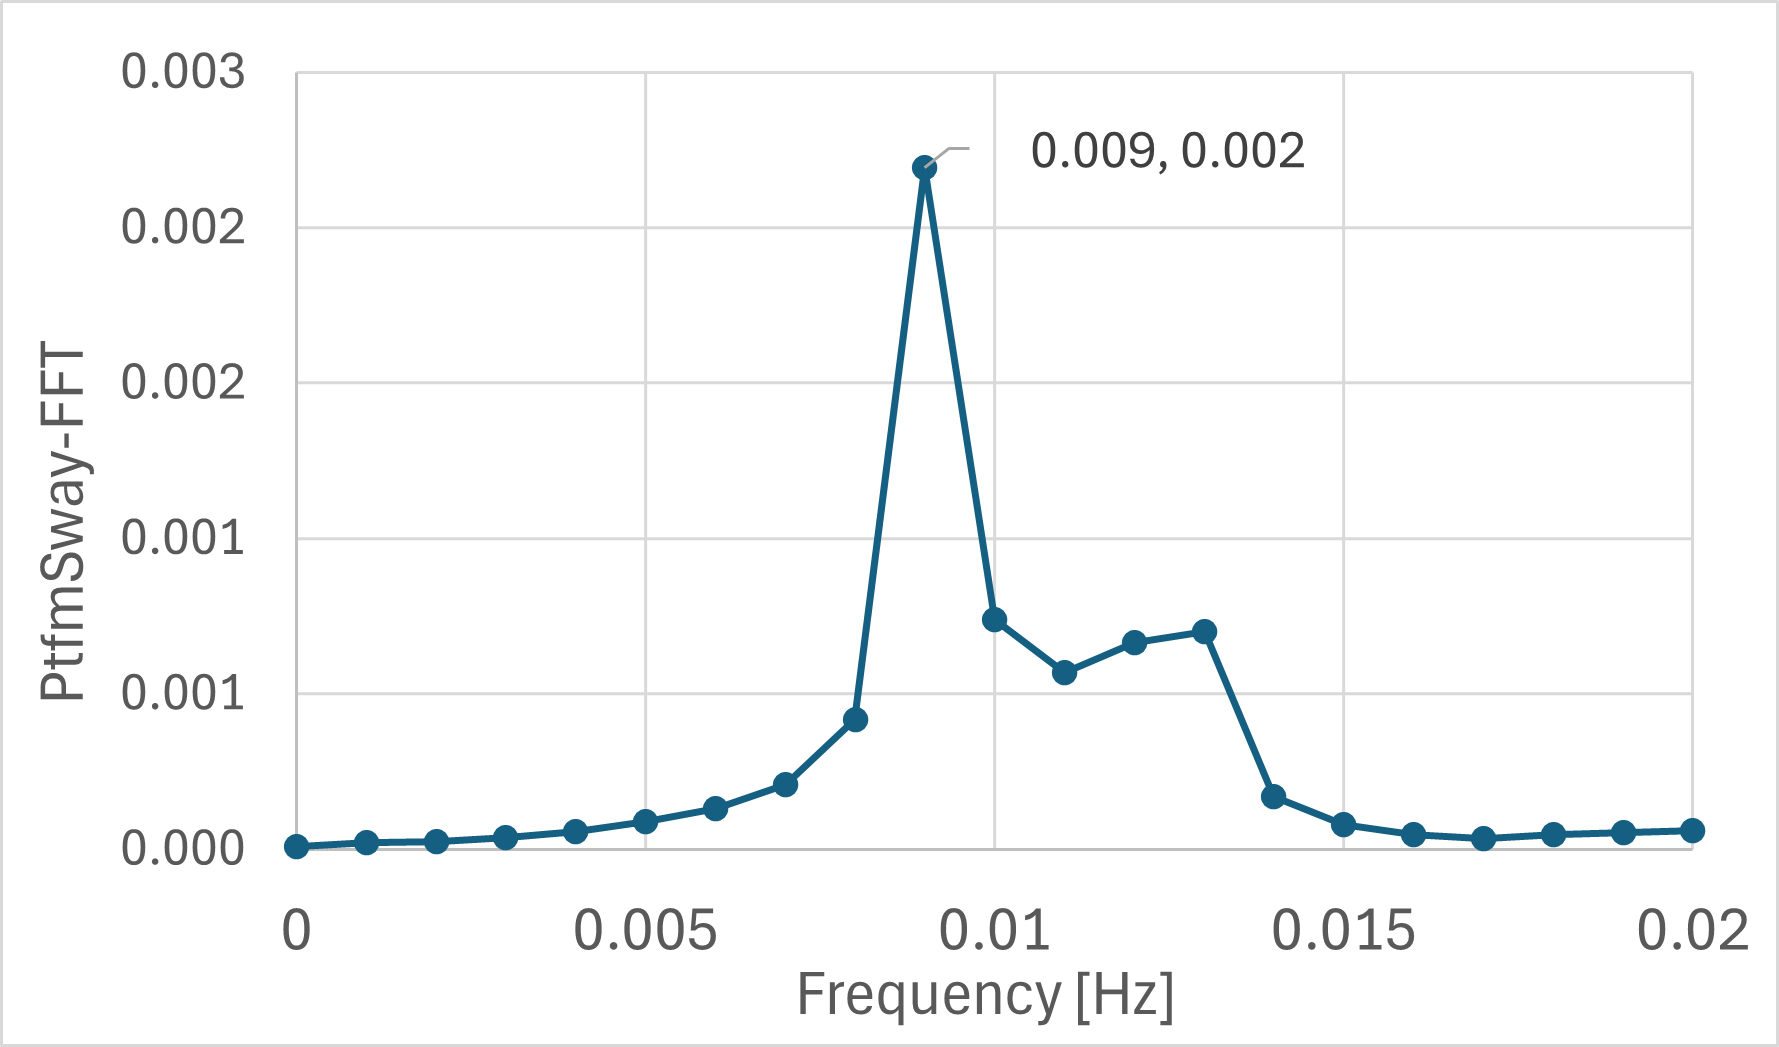
\includegraphics[width=1\textwidth]{nat_freq_sway.png}
        \caption{\small Sway natural frequency}
        \label{fig:nat_freq_sway}
    \end{minipage}
\end{figure}

\begin{figure}[H]
    \begin{minipage}{0.49\textwidth}
        \centering
        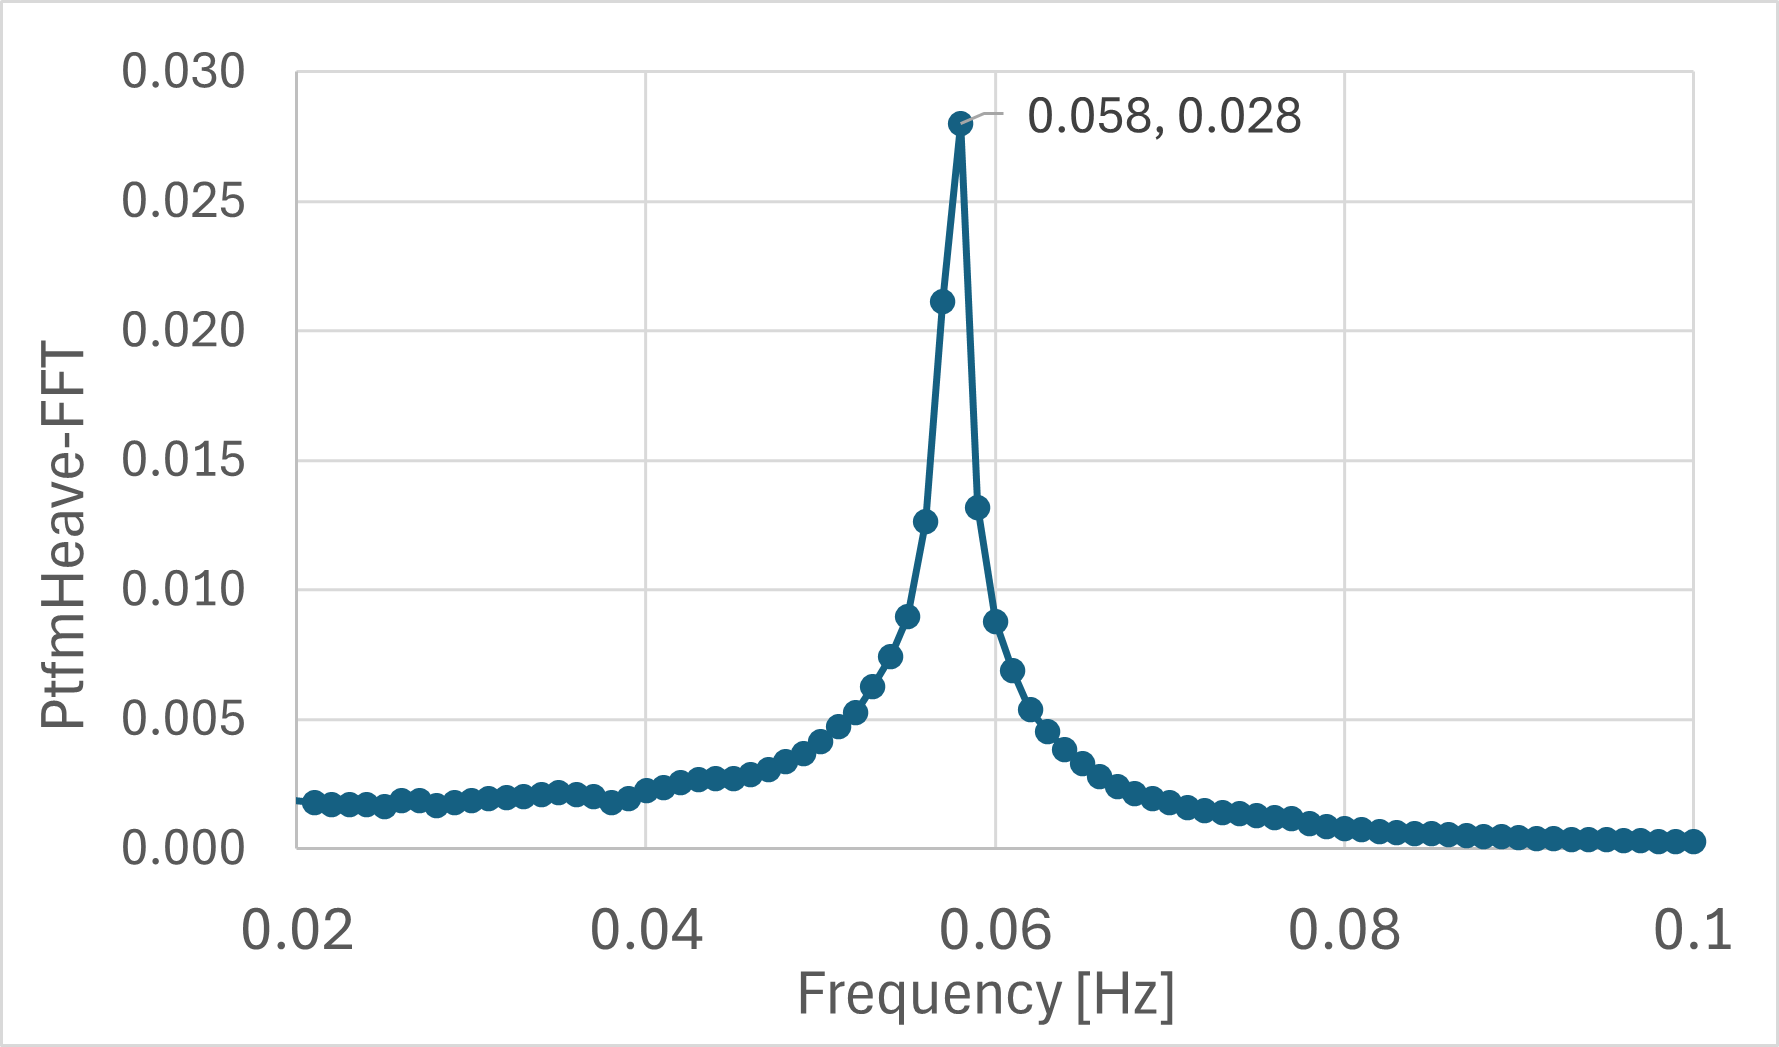
\includegraphics[width=1\textwidth]{nat_freq_heave.png}
        \caption{\small Heave natural frequency}
        \label{fig:nat_freq_heave}
    \end{minipage}
    \hfill
    \begin{minipage}{0.5\textwidth}
        \centering
        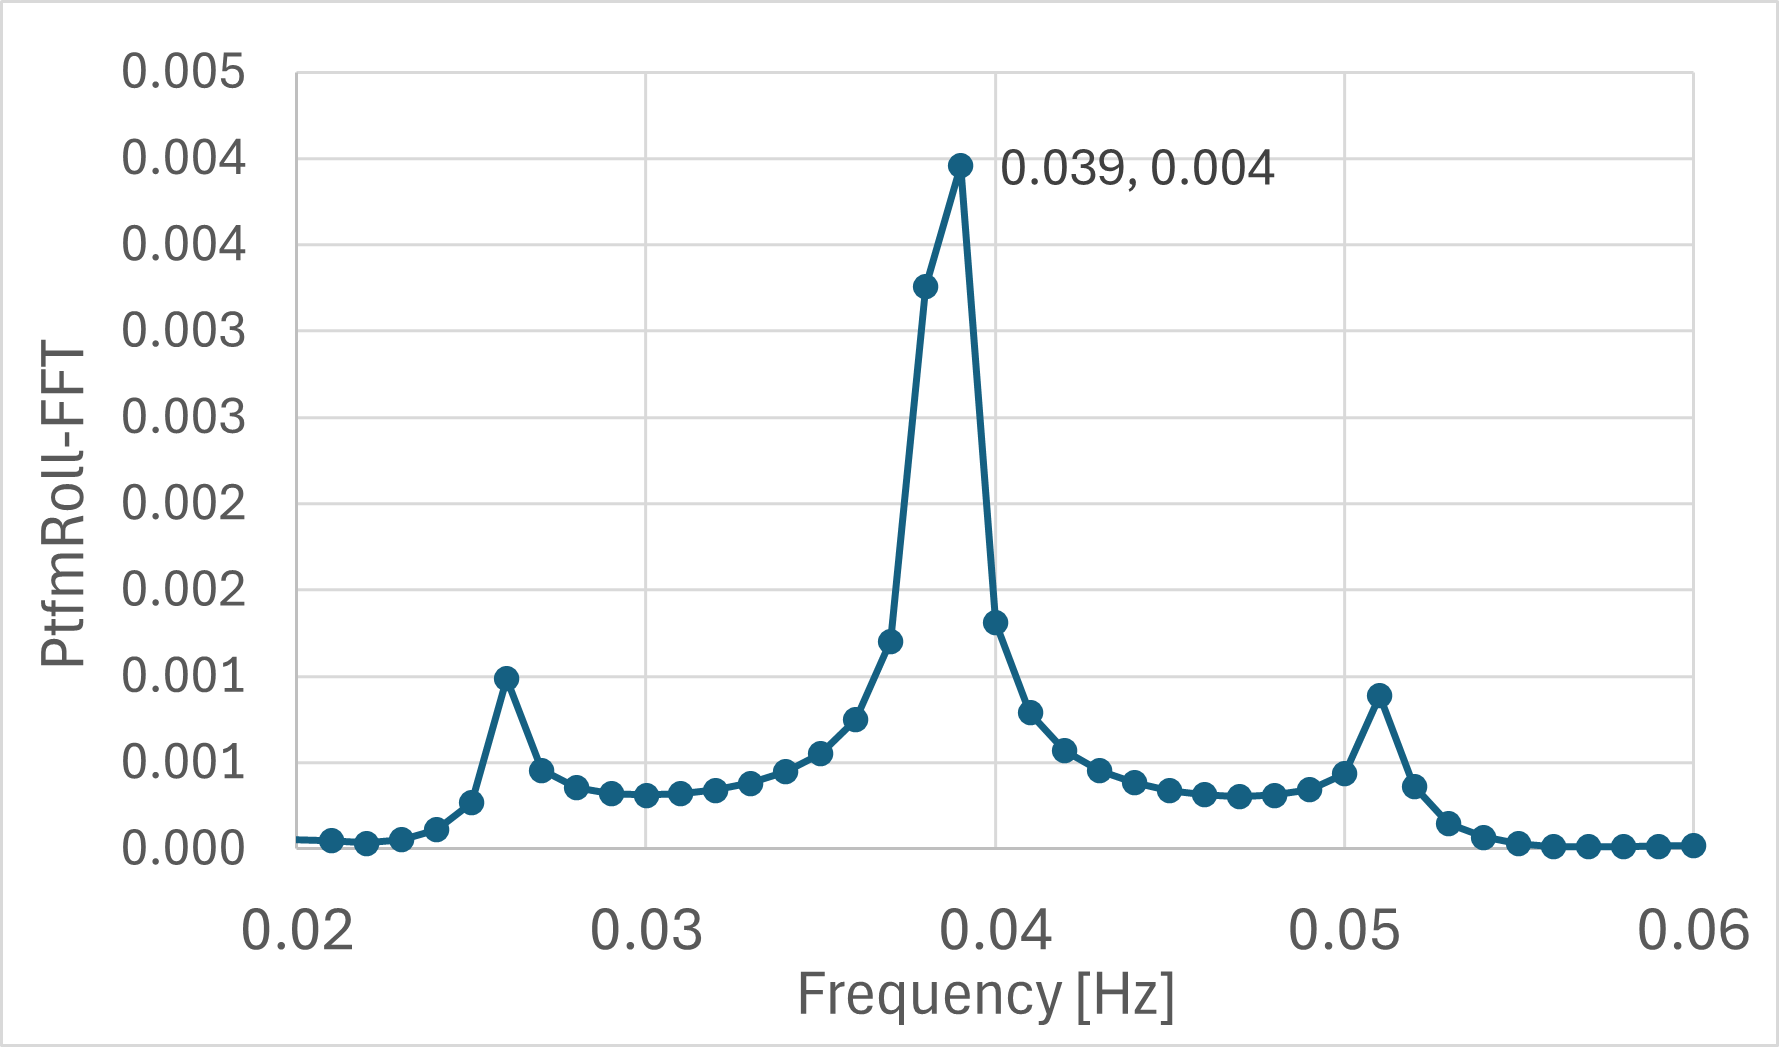
\includegraphics[width=1\textwidth]{nat_freq_roll.png}
        \caption{\small Roll natural frequency}
        \label{fig:nat_freq_roll}
    \end{minipage}
\end{figure}

\begin{figure}[H]
    \begin{minipage}{0.49\textwidth}
        \centering
        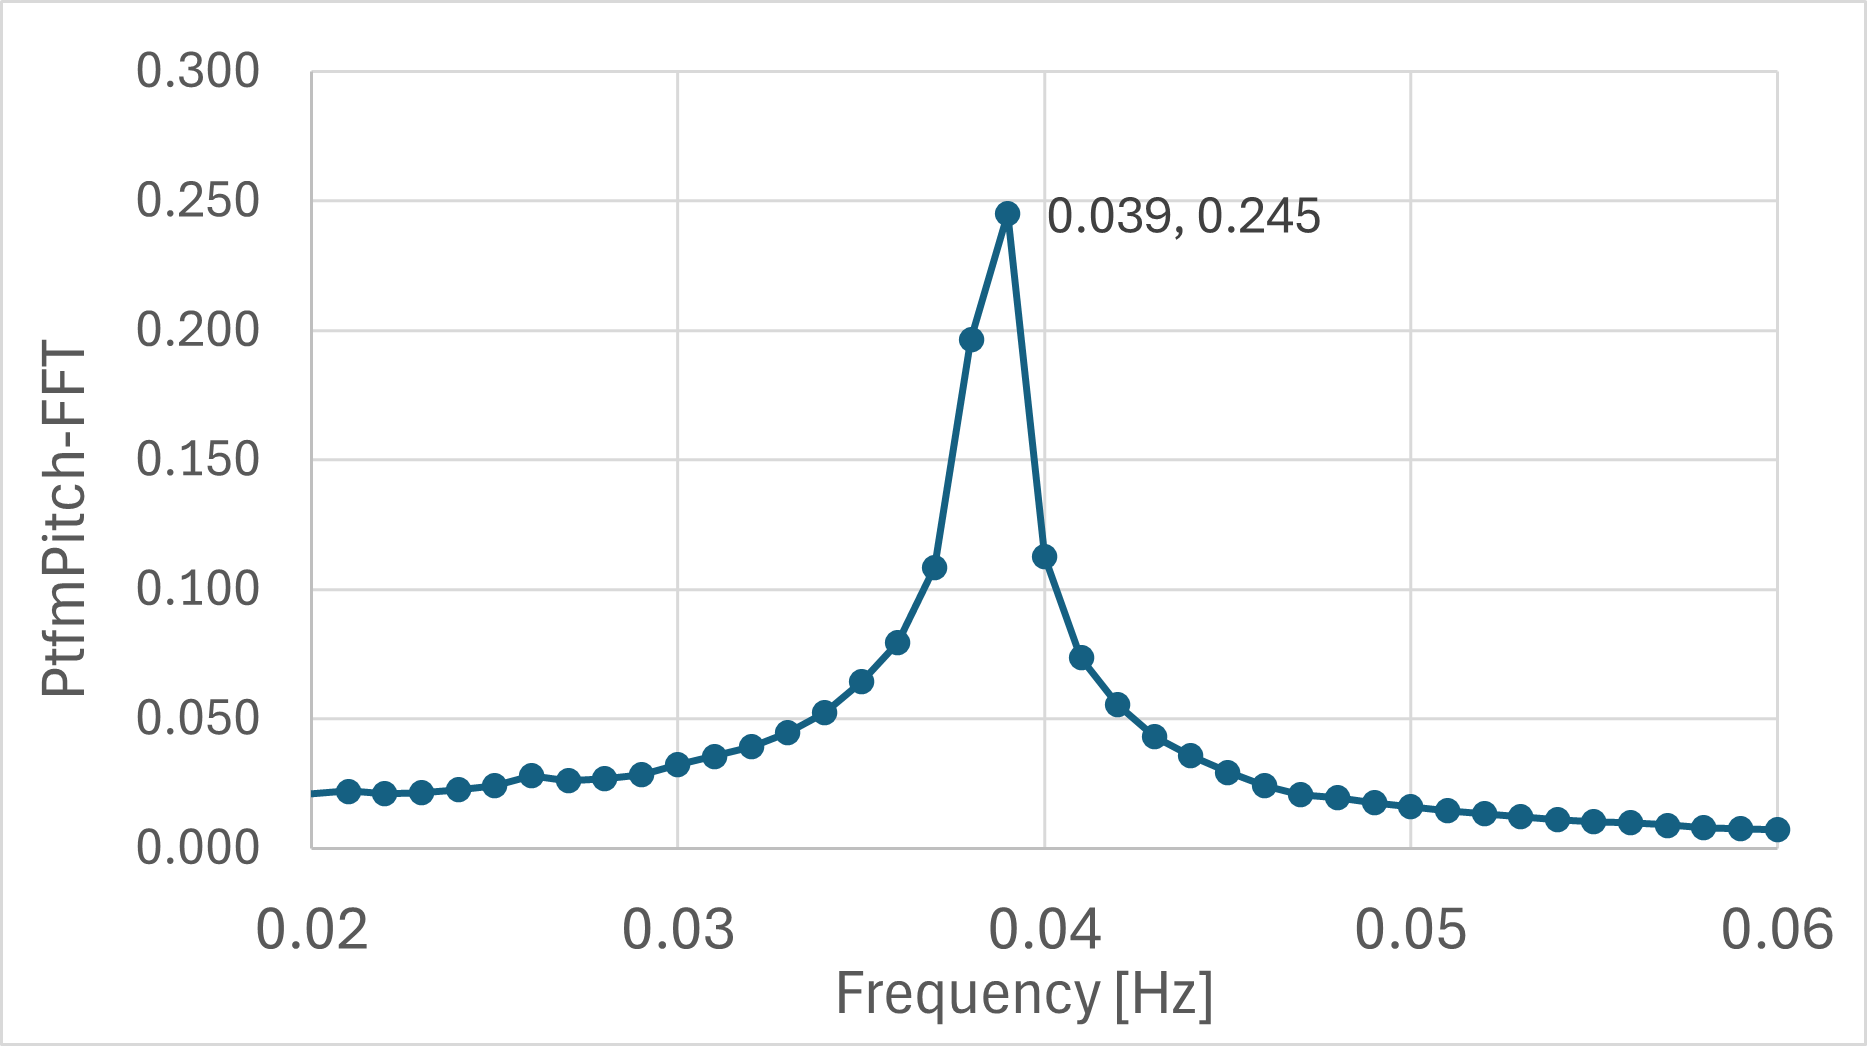
\includegraphics[width=1\textwidth]{nat_freq_pitch.png}
        \caption{\small Pitch natural frequency}
        \label{fig:nat_freq_pitch}
    \end{minipage}
    \hfill
    \begin{minipage}{0.5\textwidth}
        \centering
        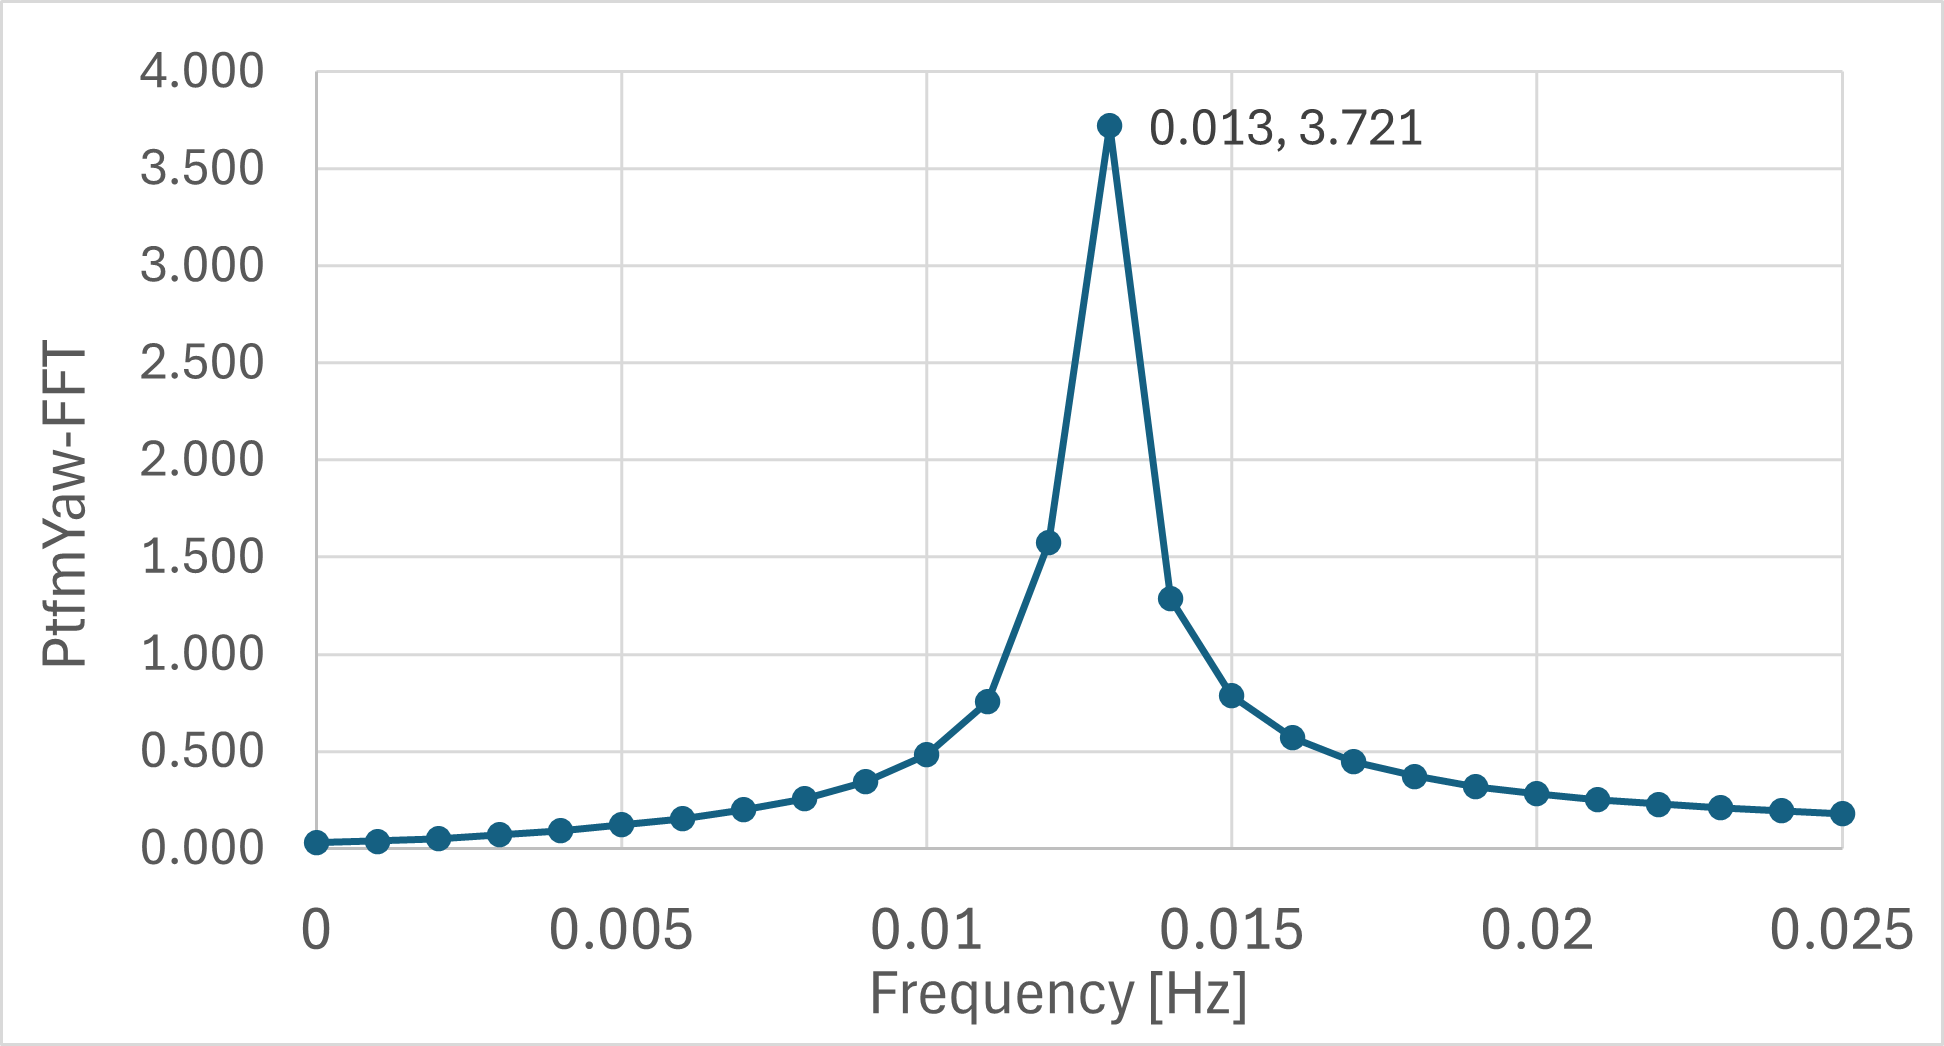
\includegraphics[width=1\textwidth]{nat_freq_yaw.png}
        \caption{\small Yaw natural frequency}
        \label{fig:nat_freq_yaw}
    \end{minipage}
\end{figure}

The natural frequency analysis of the semisubmersible platform shows a distinction in the magnitude of these frequencies across the six degrees of freedom. Specifically, the natural frequencies for heave, roll and pitch were notably higher than those for surge, sway and yaw, with heave demonstrating highest frequency overall.

This difference arises from the restoring mechanisms associated with each mode. Heave, roll, and pitch are governed by strong hydrostatic restoring forces. For heave, this is primarily due to buoyancy, where vertical displacements lead to significant changes in the buoyant force. Roll and pitch experience restoring moments due to the platform's metacentric heights, which resist angular displacements !!!!!(Jonkman, 2007) FIND BETTER REFERENCE. These restoring forces result in higher natural frequencies. In contrast, for a freely floating platform in calm water, the restoring forces for surge and sway are minimal for small displacements, leading to very low natural frequencies. Yaw experiences some hydrodynamic resistance to rotation, but this is generally weaker than the hydrostatic restoring forces in roll and pitch, resulting in a lower natural frequency compared to them. 


\subsubsection{Wave-Induced Tests}
\hspace*{0.5cm}The wave-induced responses were analyzed by applying regular and irregular waves to the platform. 


\paragraph{Load Case 2.1}
The load case 2.1 was used to analyze the platform's response to regular waves in terms of heave, pitch, and surge motions and fairlead 2 tension force. The results were processed using BEMRosetta to extract the platform's response and compared to the reference study, which can be seen in Figures 22-27. The comparison shows that the platform's response to regular waves is consistent with the reference study, specifically very similar to the NREL results for motions, confirming the accuracy of the modeling approach. The fairlead 2 tension force showed a similar trend to participants that used a dynamic mooring model, which means that this type of model treats the mooring lines as flexible structures with mass, stiffness, and damping .

%% 2.1 figures
\begin{figure}[H]
    \begin{minipage}{0.49\textwidth}
        \centering
        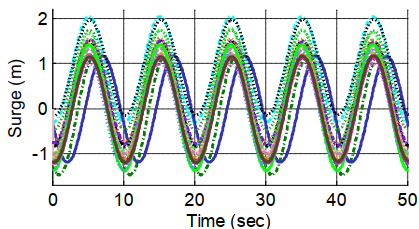
\includegraphics[width=1\textwidth]{2.1_surge.png}
        \caption{\small Surge response for 2.1 (Robertson et al., 2014)}
        \label{fig:2.1_surge}
    \end{minipage}
    \hfill
    \begin{minipage}{0.5\textwidth}
        \centering
        \vspace{-0.6cm}
        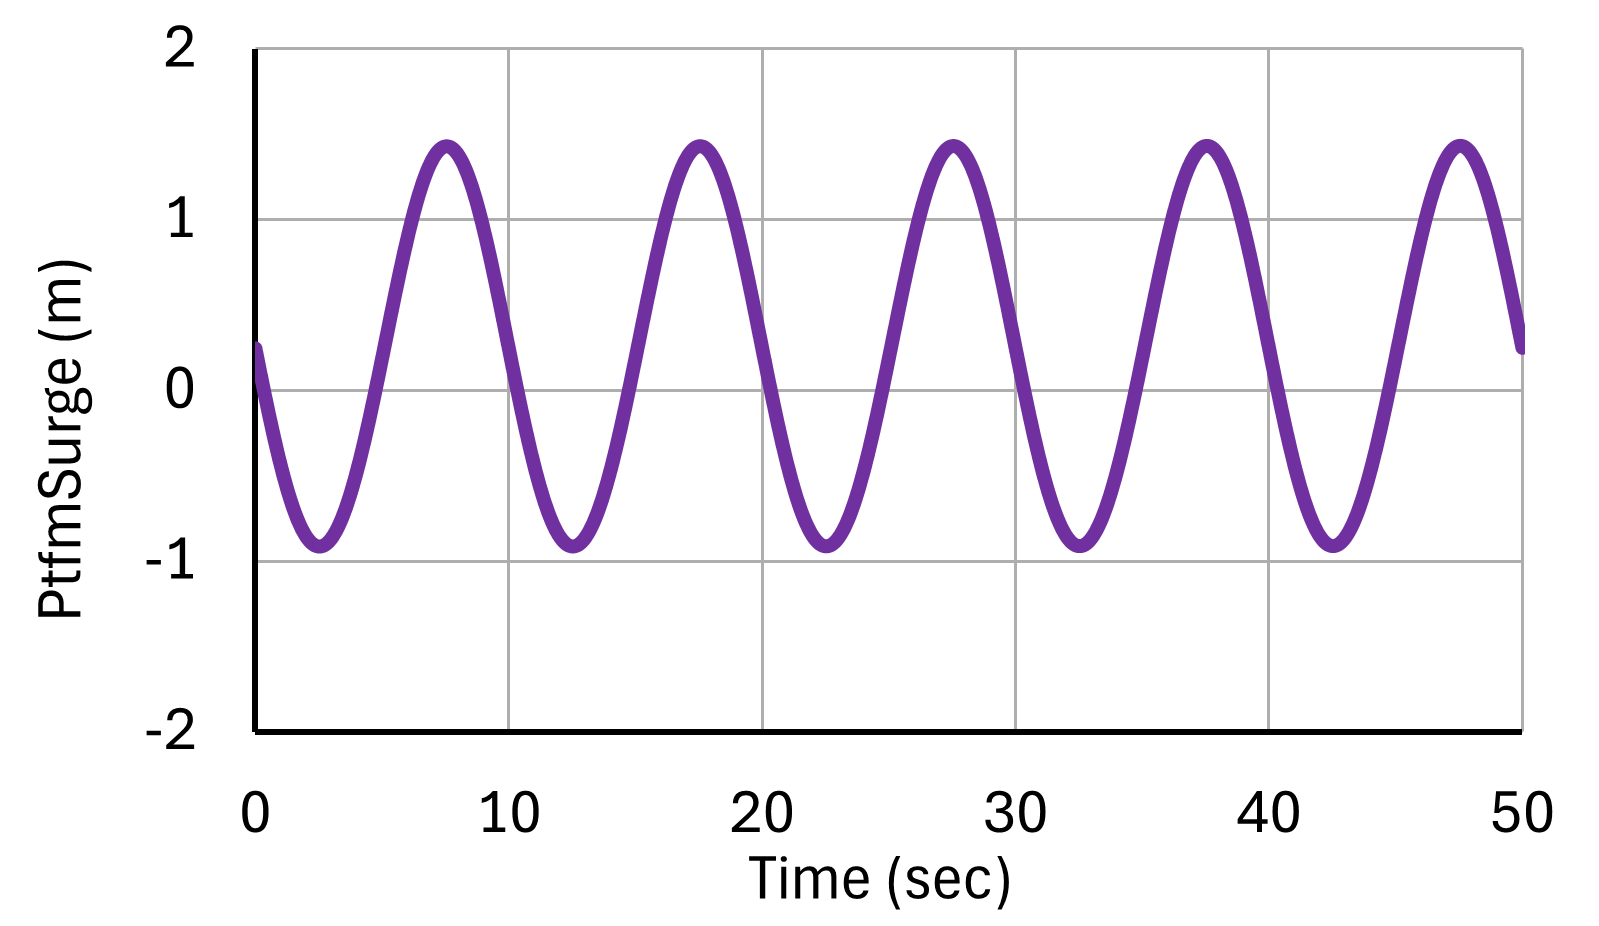
\includegraphics[width=1\textwidth]{2.1_surge_mine.png}
        \caption{\small Surge response for 2.1}
        \label{fig:2.1_surge_mine}
    \end{minipage}
\end{figure}

\begin{figure}[H]
    \begin{minipage}{0.49\textwidth}
        \centering
        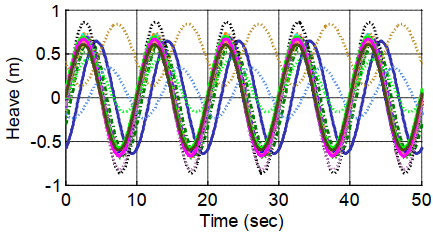
\includegraphics[width=1\textwidth]{2.1_heave.png}
        \caption{\small Heave response for 2.1 (Robertson et al., 2014)}
        \label{fig:2.1_heave}
    \end{minipage}
    \hfill
    \begin{minipage}{0.5\textwidth}
        \centering
        \vspace{-0.6cm}
        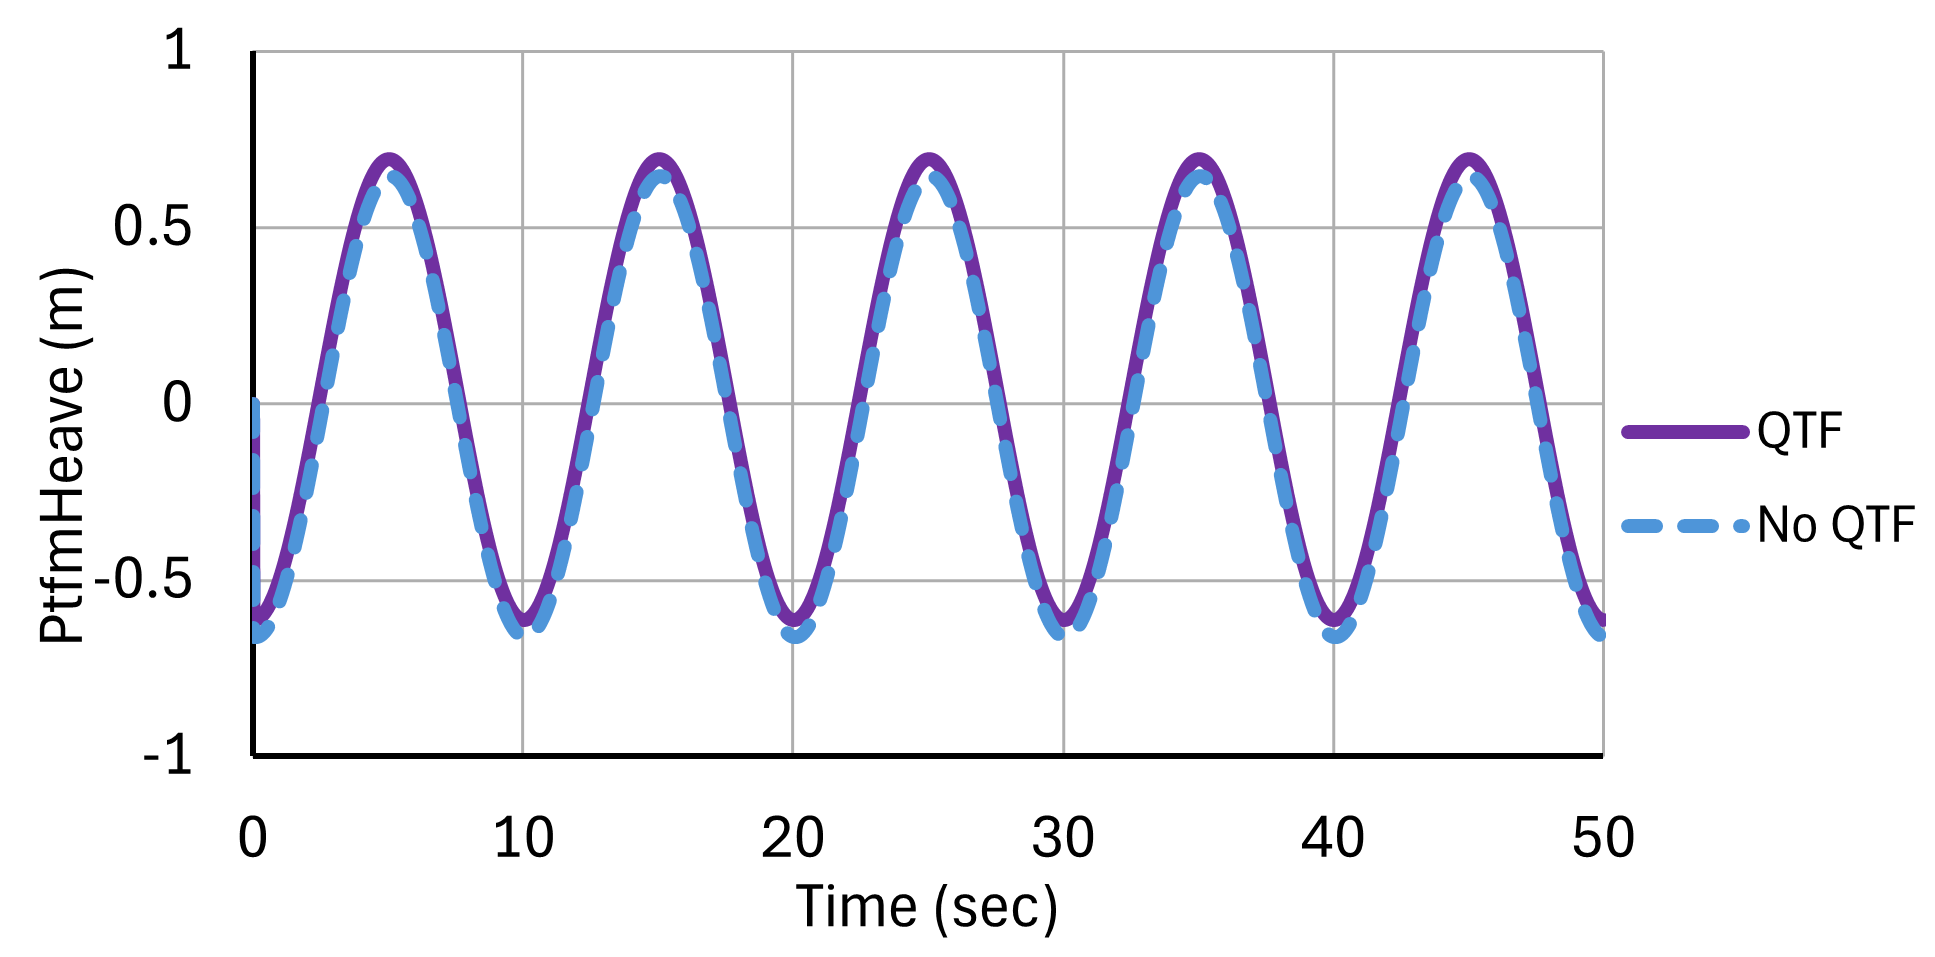
\includegraphics[width=1\textwidth]{2.1_heave_mine.png}
        \caption{\small Heave response for 2.1}
        \label{fig:2.1_heave_mine}
    \end{minipage}
\end{figure}

\begin{figure}[H]
    \begin{minipage}{0.49\textwidth}
        \centering
        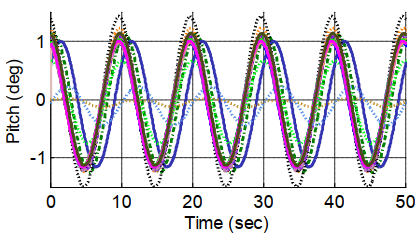
\includegraphics[width=1\textwidth]{2.1_pitch.png}
        \caption{\small Pitch response for 2.1 (Robertson et al., 2014)}
        \label{fig:2.1_pitch}
    \end{minipage}
    \hfill
    \begin{minipage}{0.5\textwidth}
        \centering
        \vspace{-0.6cm}
        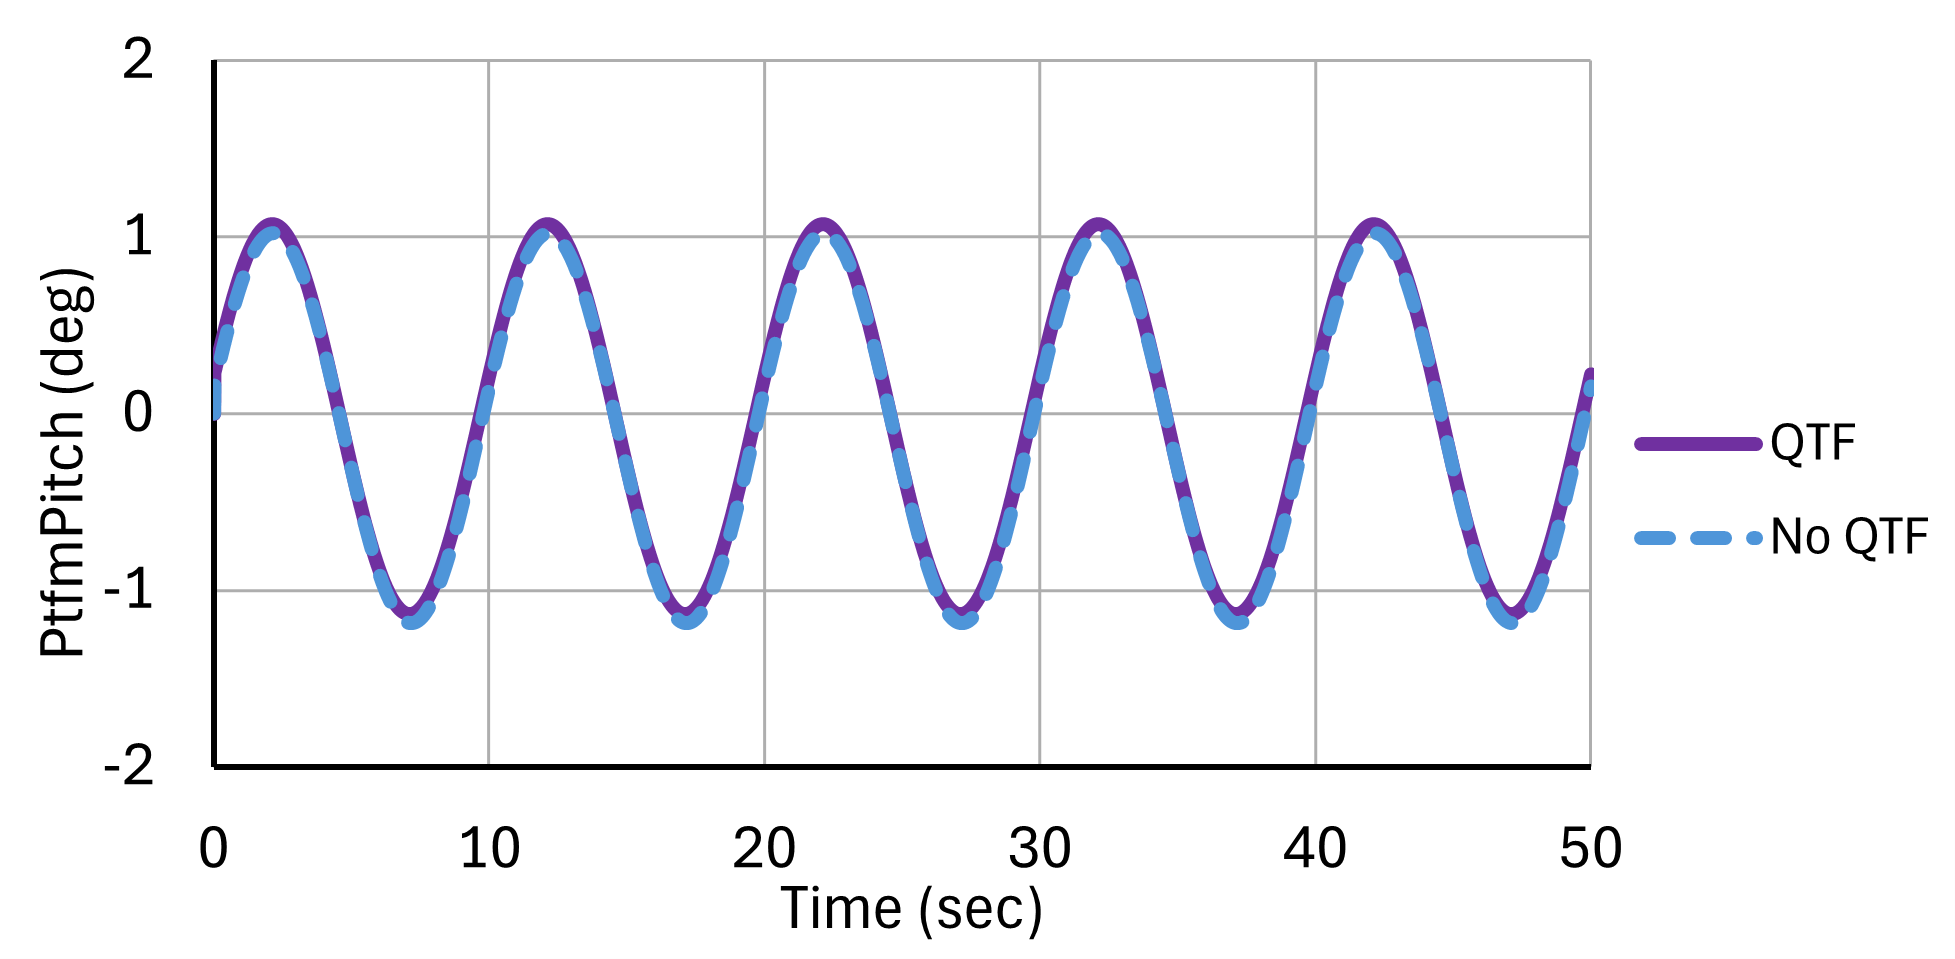
\includegraphics[width=1\textwidth]{2.1_pitch_mine.png}
        \caption{\small Pitch response for 2.1}
        \label{fig:2.1_pitch_mine}
    \end{minipage}
\end{figure}

\begin{figure}[H]
    \begin{minipage}{0.49\textwidth}
        \centering
        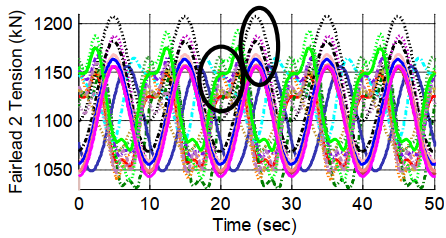
\includegraphics[width=1\textwidth]{2.1_fairten2.png}
        \caption{\small Fairlead 2 response for 2.1 (Robertson et al., 2014)}
        \label{fig:2.1_fairten2}
    \end{minipage}
    \hfill
    \begin{minipage}{0.5\textwidth}
        \centering
        \vspace{-0.6cm}
        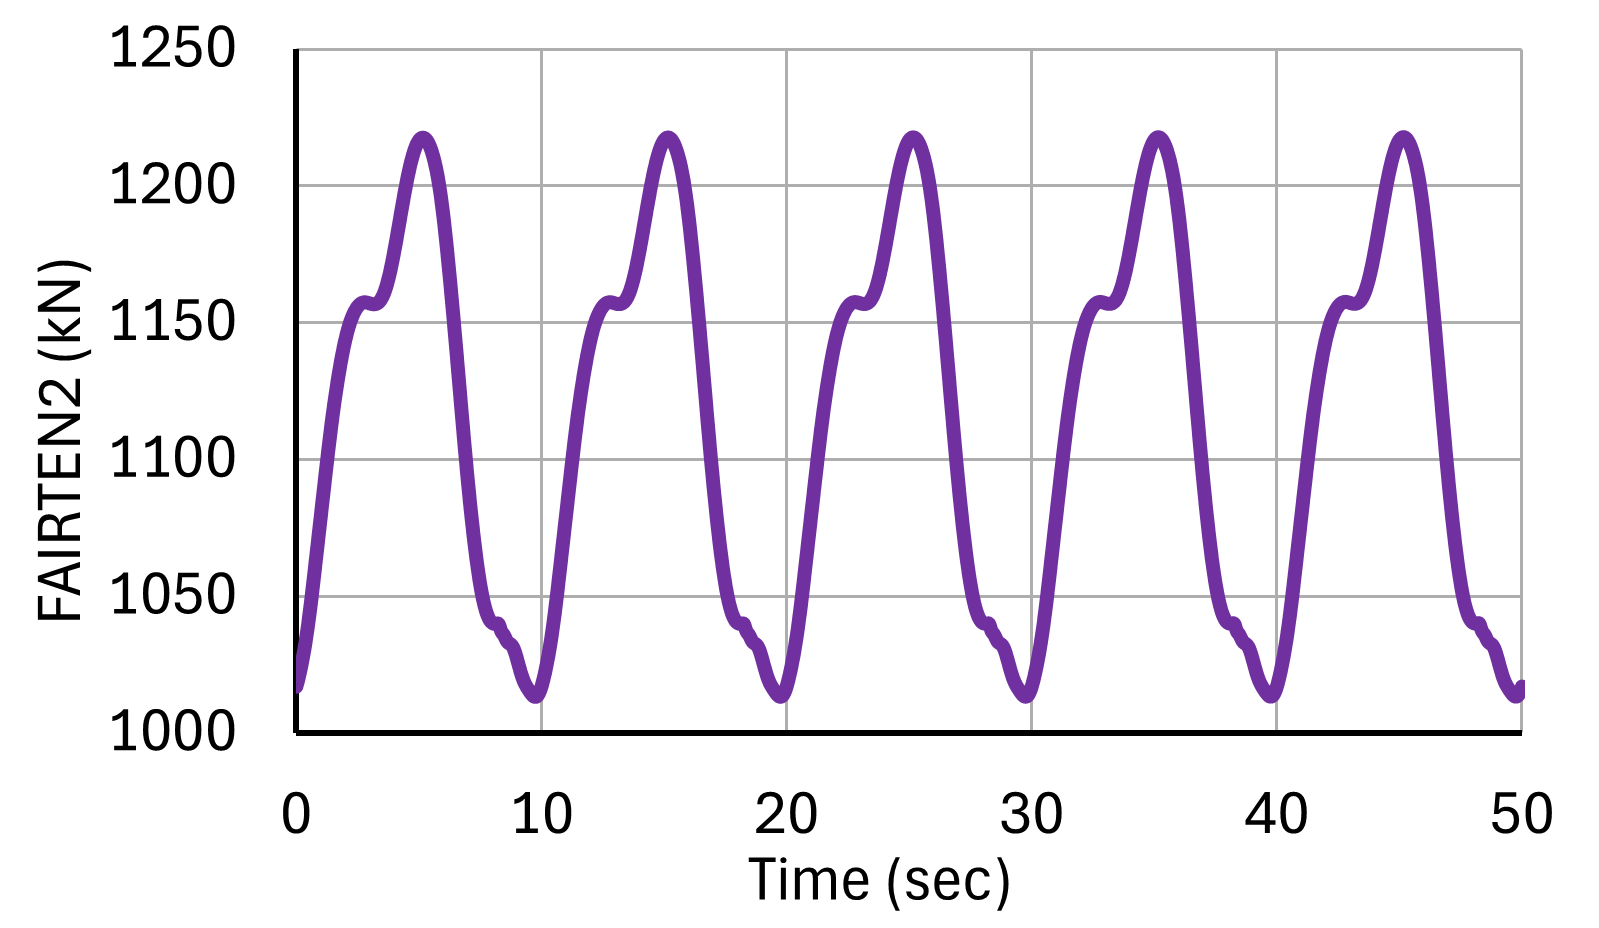
\includegraphics[width=0.95\textwidth]{2.1_fairten2_mine.png}
        \caption{\small Fairlead 2 response for 2.1}
        \label{fig:2.1_fairten2_mine}
    \end{minipage}
\end{figure}

\paragraph{Load Case 2.2}
The load case 2.2 was used to analyze the platform's response to irregular waves in terms of surge and pitch motions and tower moment. The results given in the reference study shows that the average responses to irregular waves are quite various between the participants (Figure 30). This is caused by the   

\end{document}